%%%%%%%%%%%%%%%%% CHAPTER 6 %%%%%%%%%%%%%%%%%%%%%%%%%%%%%%%%%
%%%%% Sorting %%%%%%%%%%%%%%%%%%%%%%%%%%%%%%%%%%%%%%%%%%%%%%%%
\section{Flow in Porous Materials}
Flow in porous media is a topic that appears in many branches of engineering and science, e.g., ground water hydrology, reservoir engineering, soil science, soil mechanics, and chemical engineering (filtration).
The aquifer, which is the porous medium domain of the hydrologist, or the oil reservoir, which is the porous medium of the petroleum engineer are typical examples.

Figure \ref{fig:aquifers} is a sketch of different aquifer classifications. 
A confined aquifer (pressure aquifer) is one bounded above and below by impermeable formations.
In a well penetrating such an aquifer, the water level will rise above the base of the confining formation.
Water levels in wells that sample a certain aquifer define an imaginary surface called the piezometric surface.

\begin{figure}[h!] %  figure placement: here, top, bottom, or page
   \centering
   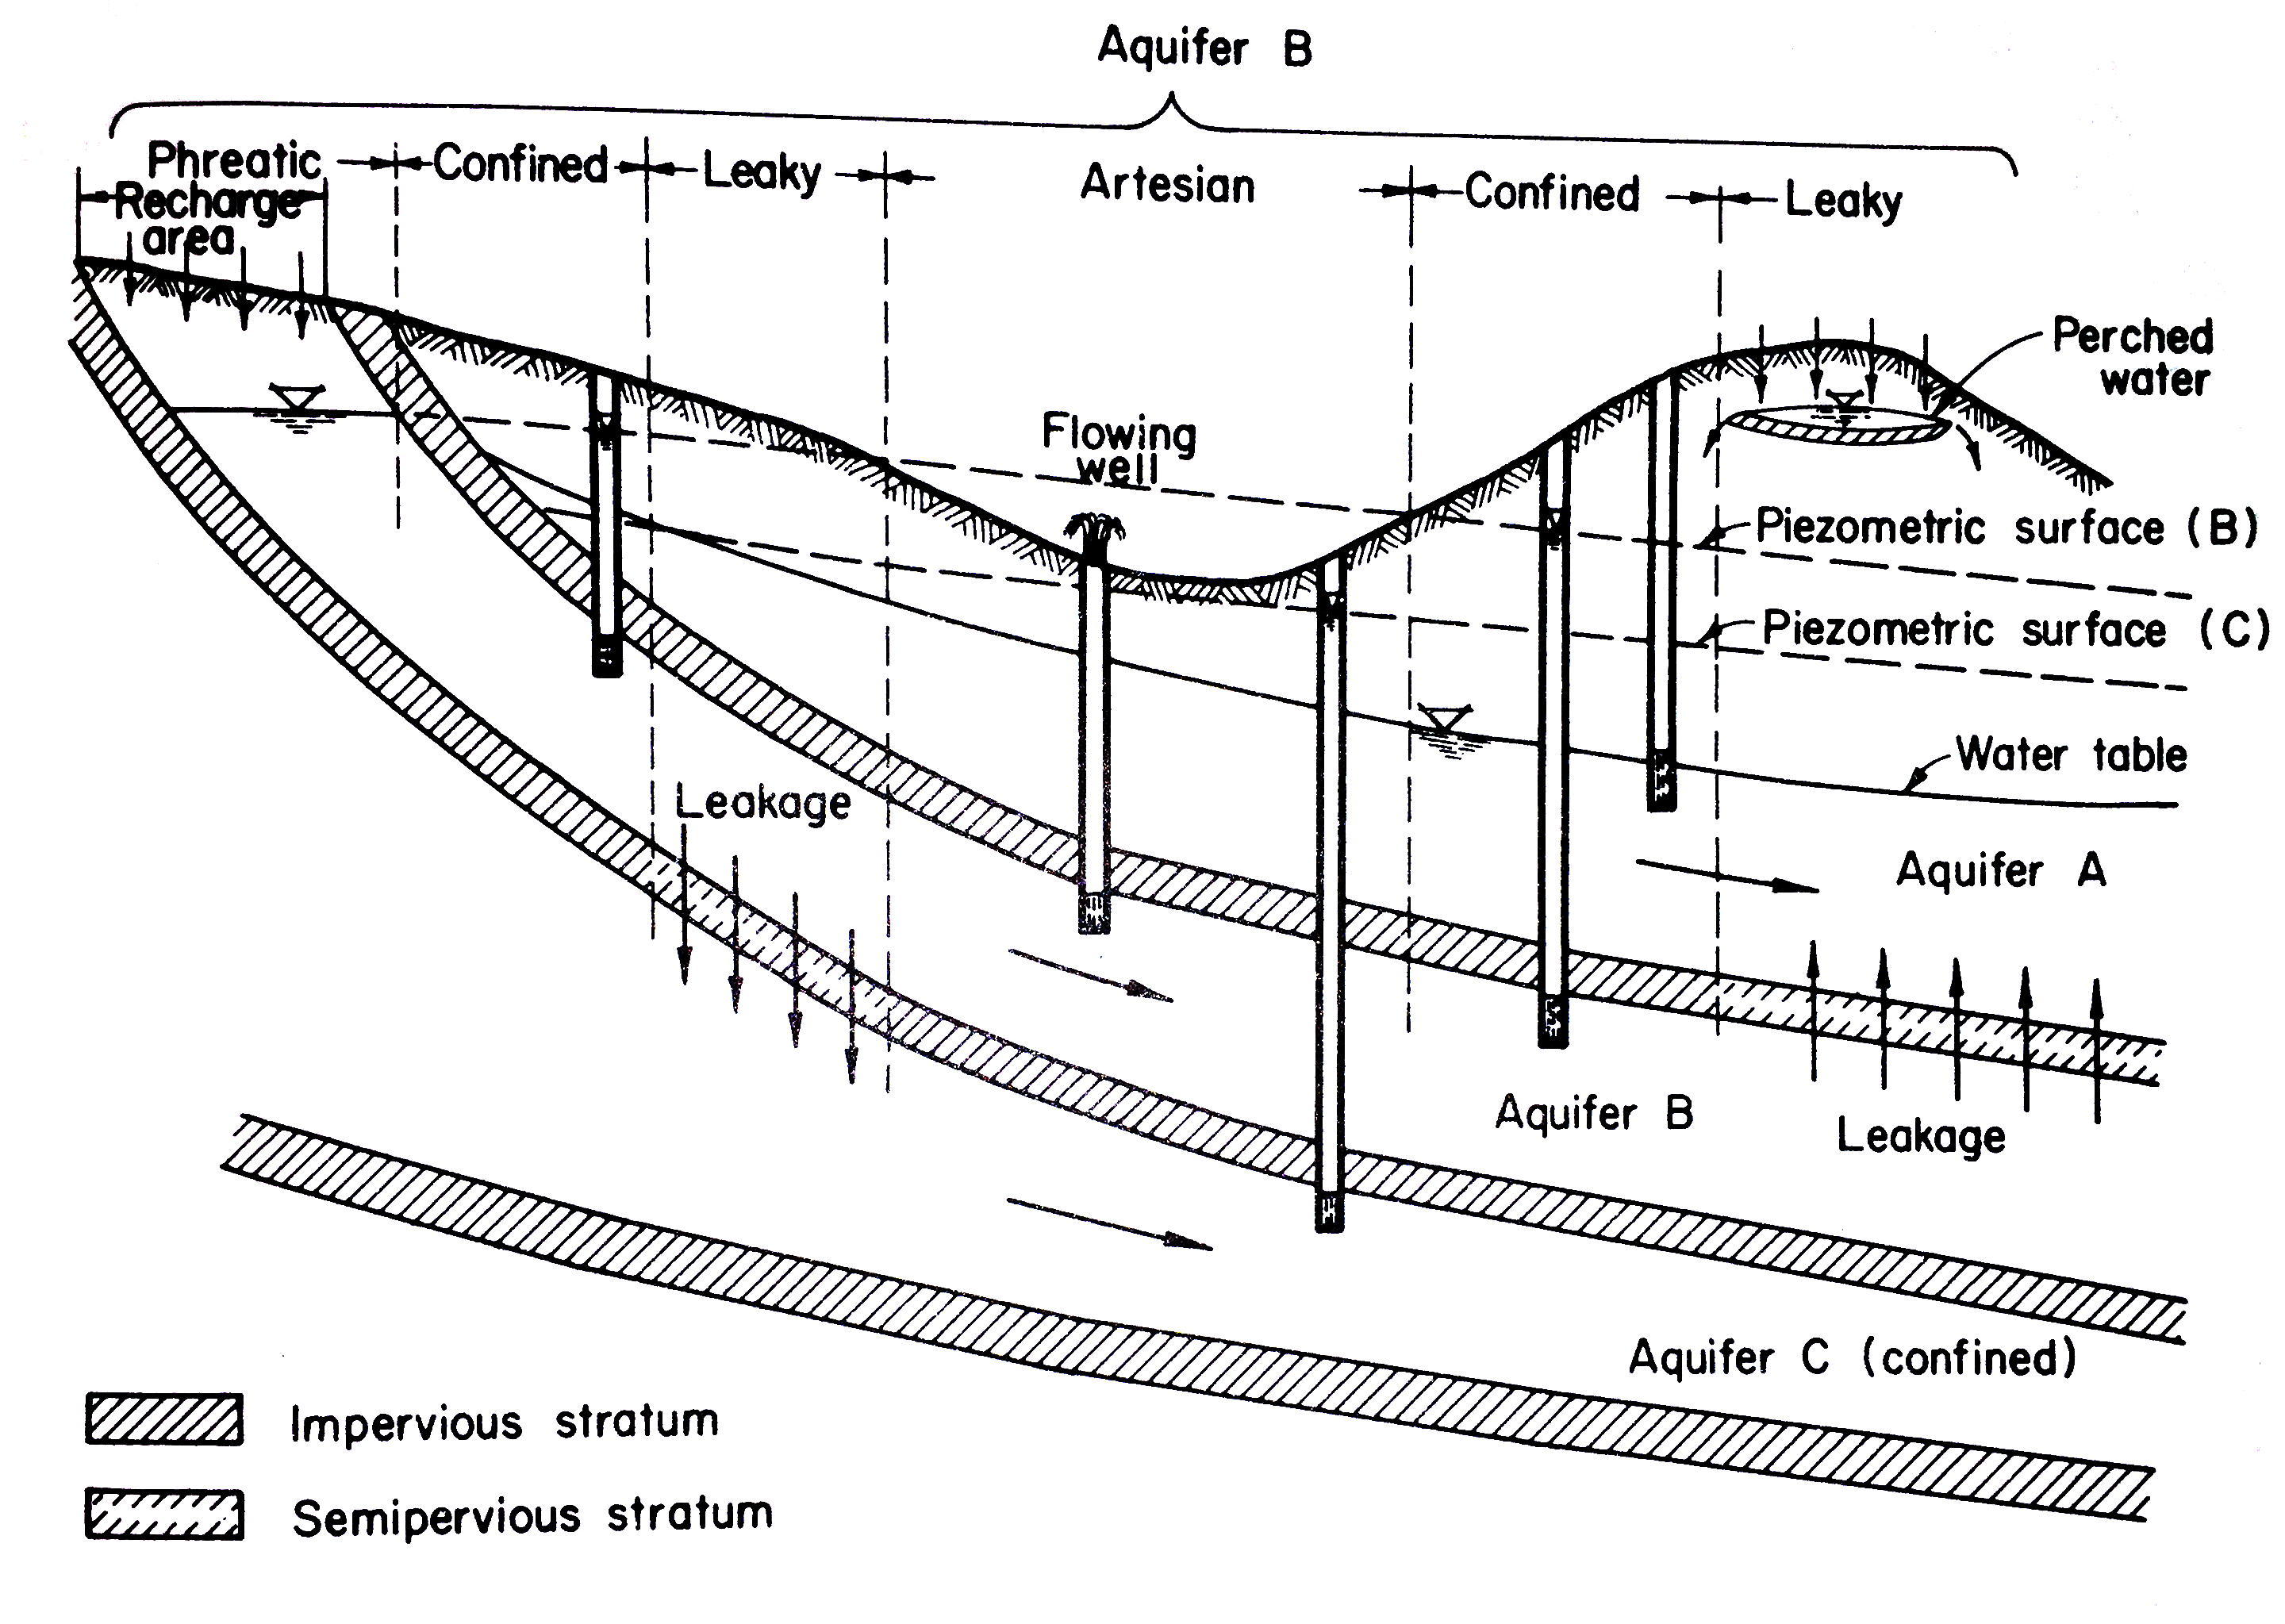
\includegraphics[width=6in]{./14-PorousMediumFlow/aquifers.jpg} 
   \caption{Aquifer classifications}
   \label{fig:aquifers}
\end{figure}

An unconfined aquifer (water table aquifer; phreatic aquifer) is one with the water table as its upper boundary.
The classifications are important because the equations of motion are different in different kinds of aquifers.

\subsection{Storage}
Storativity of an aquifer is the relationship between changes in head within the aquifer and the quantity of water stored in the aquifer.
Figure \ref{fig:storage} is a sketch showing the storage process in a confined, and unconfined aquifer.
\begin{figure}[h!] %  figure placement: here, top, bottom, or page
   \centering
   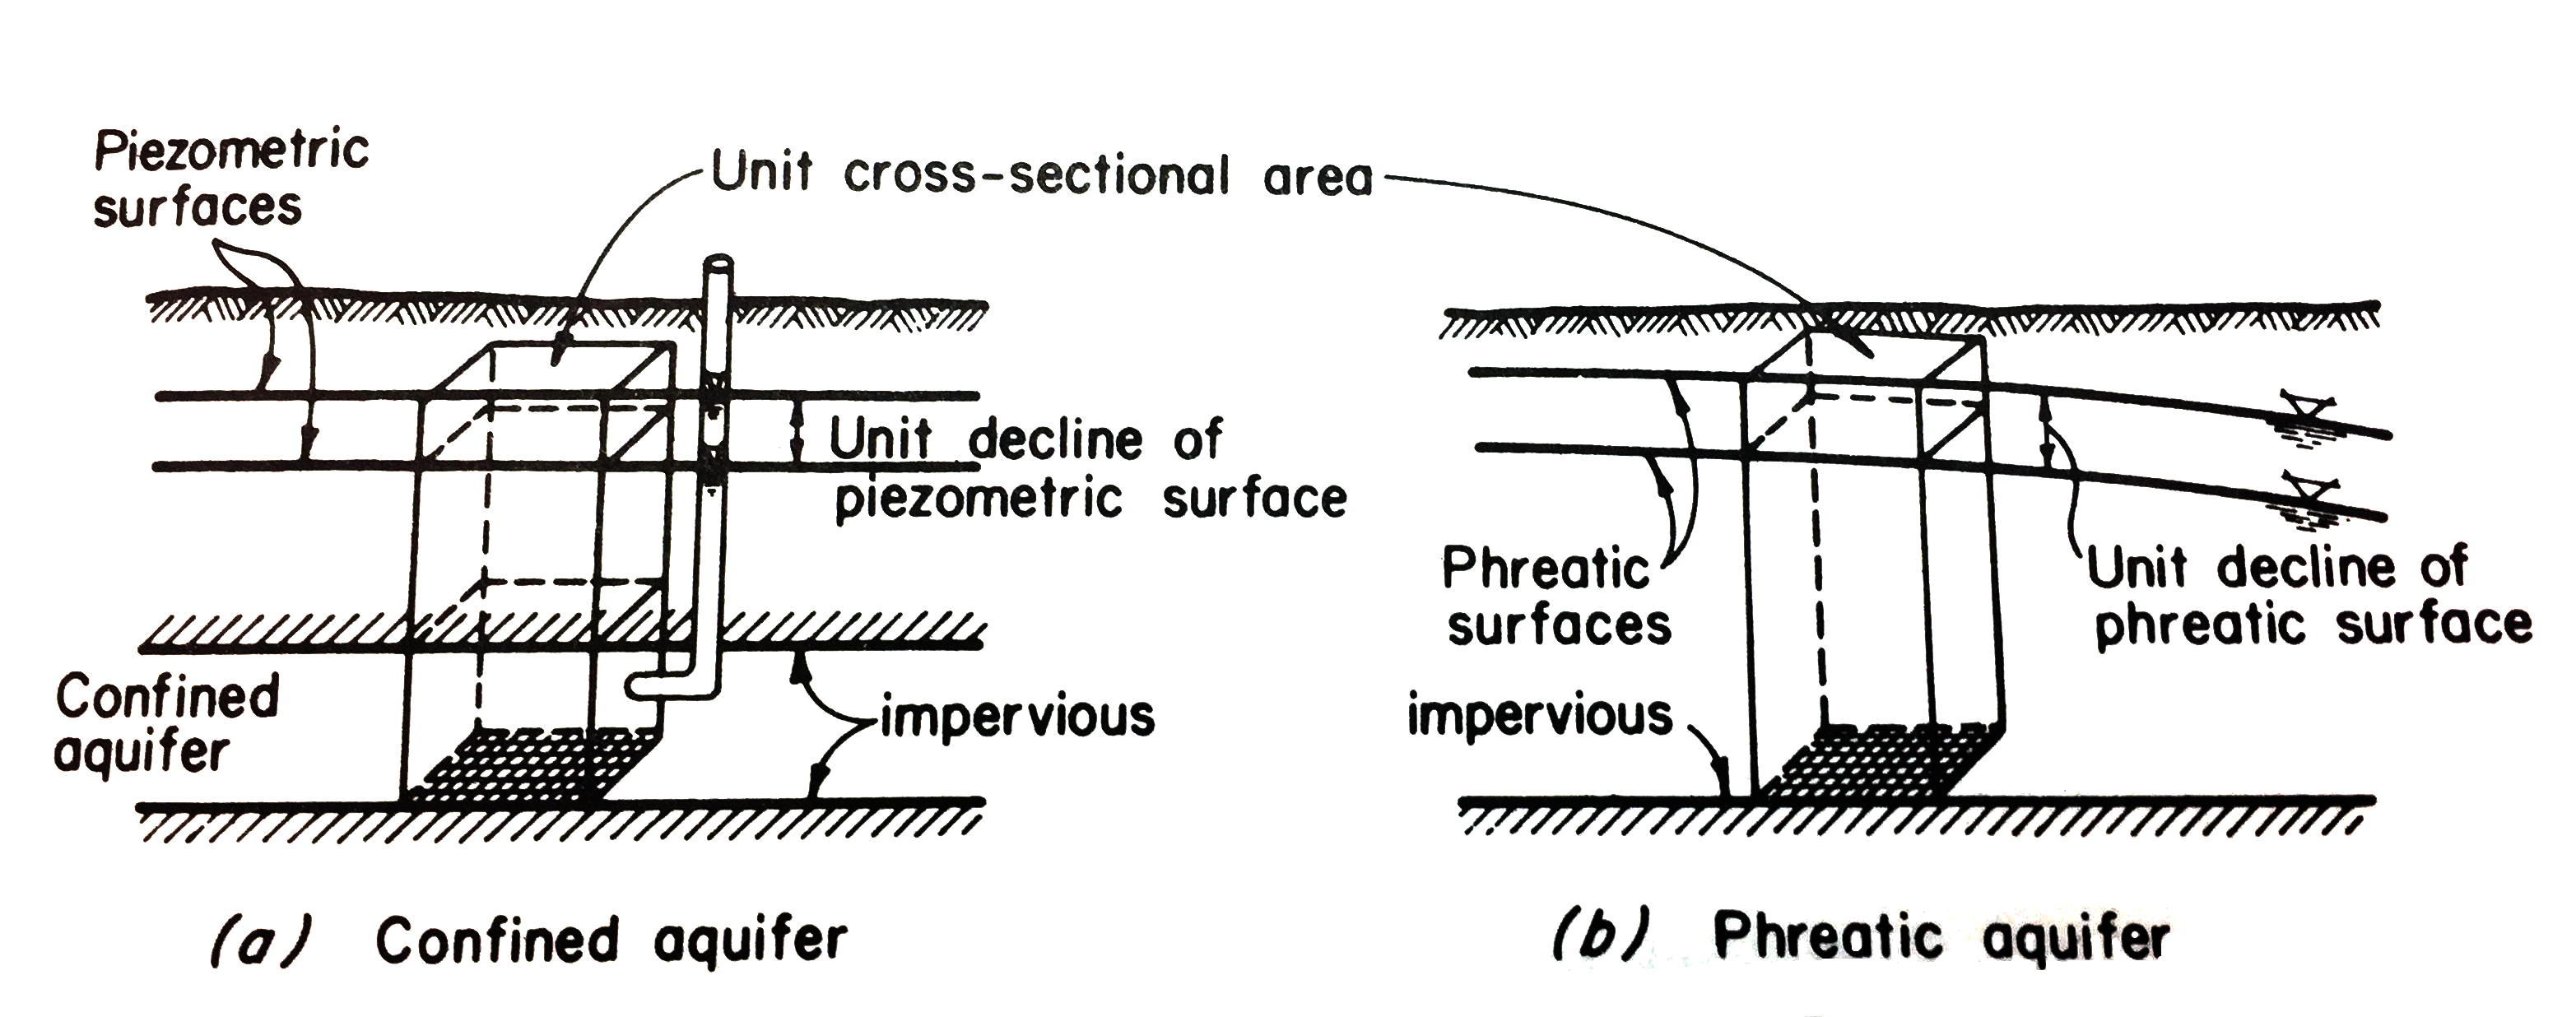
\includegraphics[width=6in]{./14-PorousMediumFlow/storage.jpg} 
   \caption{Illustrative sketches of definition of storage coefficient}
   \label{fig:storage}
\end{figure}
\newline
The mechanism of storage is different for confined and unconfined aquifers.
In a confined aquifer the water is stored or released by compression and decompression of water and the solid matrix (like a sponge squeezed while wrapped in plastic wrap).
In an unconfined aquifer the water is stored or released from the pore space when the water table elevation changes.

The storage coefficient (confined) or specific yield (unconfined) is the volume of water added to (or removed from) storage per unit area of aquifer per unit change in head.  The usual symbols are $S$, and $S_y$.


\subsection{Permeability}
Permeability is the material property that relates the resistance of flow through the porous medium to the hydraulic gradient.

\subsection{Head Loss Models}
Darcy's law (a linear flux model) is the head loss model used for porous media flow.   
Equation \ref{eqn:darcy-law} is Darcy's law expressed as a head loss model.
\begin{equation}
h_L = \frac{QL}{KA}
%Q = KA\frac{\partial h}{\partial x}
\label{eqn:darcy-law}
\end{equation}
where $Q$ is the discharge in the aquifer, $L$ is the length in the flow direction, $A$ is the cross sectional area of aquifer (pore space and solid phase), $K$ is the hydraulic conductivity.\footnote{also called the permeability}

A more useful (for computation) form of the head loss model, is to express it [the loss equation] as an equation of motion as in Equation \ref{eqn:groundwater-motion}.
\begin{equation}
Q = -KA\frac{\partial h}{\partial x}
\label{eqn:groundwater-motion}
\end{equation}
where $- \frac{\partial h}{\partial x}$ is the hydraulic gradient (slope of the hydraulic grade line) in the aquifer.

Figure \ref{fig:1D-aquifer-flow} is a diagram that illustrates the relationships expressed by Darcy's law.  

\begin{figure}[h!] %  figure placement: here, top, bottom, or page
   \centering
   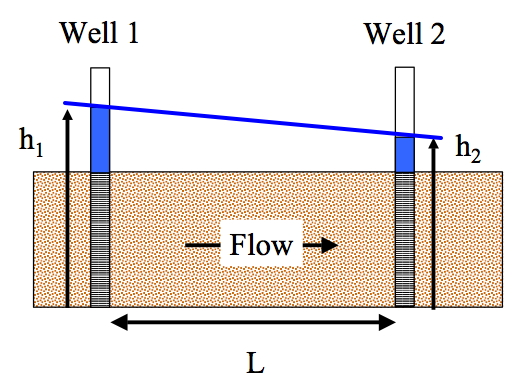
\includegraphics[width=6in]{./14-PorousMediumFlow/1D-aquifer-flow.jpg} 
   \caption{Schematic diagram of unidirectional flow in a generic aquifer, showing heads in two measuring wells located distance $L$ apart.}
   \label{fig:1D-aquifer-flow}
\end{figure}

The cross-sectional flow area, $A$, is the product of height of the aquifer block and its width [in this case the width is into the plane of the paper].
The distance between two measurement points is $L$.
The head at the two points is $h_1$ and $h_2$.
The gradient of head, $\frac{\partial h}{\partial x}$, is $\frac{h_2 - h_1}{L}$.
The hydraulic gradient is  $- \frac{\partial h}{\partial x}$, is $\frac{h_1 - h_2}{L}$.
Finally Darcy's law (for the drawing) is $Q = K A \frac{h_1 - h_2}{L}$.

\subsection{Confined Aquifer Flow}
Using Figure \ref{fig:1D-aquifer-flow} as a starting point, we can develop a computational model of flow in a confined aquifer.
Let's decide that the distance $L$ in the figure is going to be divided into a series of connected, small blocks.
The flow direction in the figure will be declared the $x$ direction, the depth into the drawing is declared the $y$ direction, and the height of the block is declared the $z$ direction.

Figure \ref{fig:single-computational-cell} is a diagram of one such small block.
\begin{figure}[h!] %  figure placement: here, top, bottom, or page
   \centering
   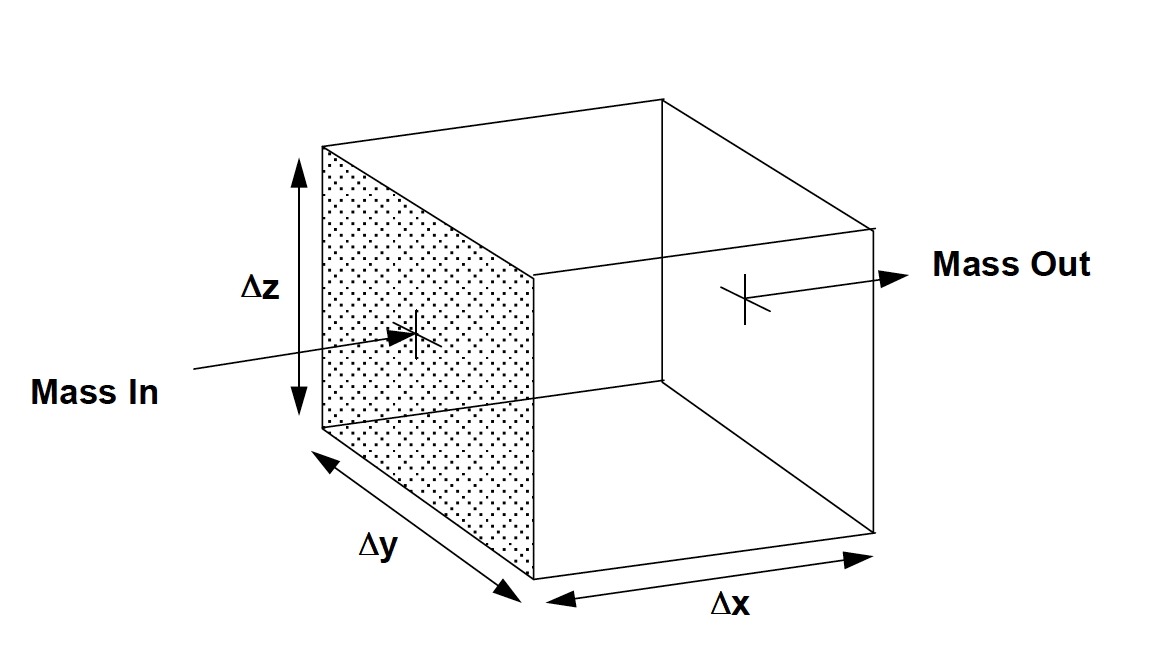
\includegraphics[width=6in]{./14-PorousMediumFlow/single-computational-cell.jpg} 
   \caption{Single computational cell definition sketch}
   \label{fig:single-computational-cell}
\end{figure}

Using this diagram we can now develop a set of expressions for the cell volume, solids volume in the cell,  pore volume in the cell (where water actually can flow), and solids mass.

\begin{equation}
V_{cell} = \Delta x \times \Delta y \times \Delta z
\end{equation}

\begin{equation}
V_{soild} =(1-\omega) \Delta x \times \Delta y \times \Delta z
\end{equation}

\begin{equation}
V_{pore} = \omega \Delta x \times \Delta y \times \Delta z
\end{equation}

\begin{equation}
M_{solid} = \rho_{s} (1-\omega) \Delta x \times \Delta y \times \Delta z
\end{equation}

Next write a mass balance for water in the cell;
\begin{equation}
\frac{d M_{water}}{dt} = M_{Inflow} - M_{Outlfow}
\end{equation}

The left side of the expression is simply the storage term, and in the context of storage coefficients and aquifer head is replaced by
\begin{equation}
{\frac{d M_{water}}{dt}\mid}_{cell} =\rho_{w} S_{s} \Delta x \Delta y \Delta z \frac{\partial h_i}{\partial t}
\end{equation}
 where $h_i$ is the head in the $i-$th cell.  
 
The right hand side of the expression is based on writing Darcy's law for the cell, using values in adjacent (hydraulically connected) cells.

\begin{figure}[h!] %  figure placement: here, top, bottom, or page
   \centering
   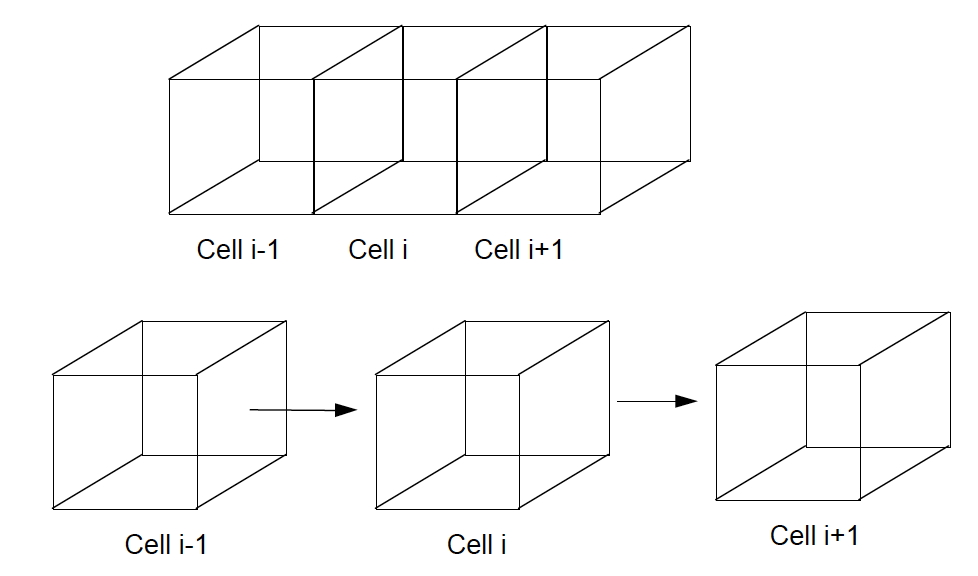
\includegraphics[width=6in]{./14-PorousMediumFlow/multiple-computational-cell.jpg} 
   \caption{Multiple computational cell definition sketch}
   \label{fig:multiple-computational-cell}
\end{figure}

Figure \ref{fig:multiple-computational-cell} is a sketch showing three such cells.  
The $i-$th cell is the cell of interest, the cell to the left is cell ID $i-1$, and the cell to the right is cell ID $i+1$.  

We now write Darcy's law for each face of cell $i$, treating the head in each of the cell centers as if they were the sampling wells of Figure \ref{fig:1D-aquifer-flow}.\footnote{In the context of Figure \ref{fig:1D-aquifer-flow}, the cell face is halfway between the two wells; the cell centers are at the wells.}

Darcy's law for the left face is 

\begin{equation}
M_{Inflow} = Q_{left} =\rho_{w} K \Delta y \Delta z \frac{h_{i-1} - h_{i}}{\Delta x}
\end{equation}
 
Similarly for the right face, 
 \begin{equation}
M_{Outflow} = Q_{right} =\rho_{w} K \Delta y \Delta z \frac{h_{i} - h_{i+1}}{\Delta x}
\end{equation}

Now combine these together in the mass balance
 \begin{equation}
\rho_{w} S_{s} \Delta x \Delta y \Delta z \frac{\partial h_i}{\partial t} = 
(\rho_{w} K \Delta y \Delta z \frac{h_{i-1} - h_{i}}{\Delta x}) - 
(\rho_{w} K \Delta y \Delta z \frac{h_{i} - h_{i+1}}{\Delta x})
\end{equation}

Next divide by the water density $\rho_{w}$,
 \begin{equation}
S_{s} \Delta x \Delta y \Delta z \frac{\partial h_i}{\partial t} = 
(K \Delta y \Delta z \frac{h_{i-1} - h_{i}}{\Delta x}) - 
(K \Delta y \Delta z \frac{h_{i} - h_{i+1}}{\Delta x})
\label{eqn:finite-difference-structure}
\end{equation}

The divide by cell width $\Delta y $,
 \begin{equation}
S_{s} \Delta x \Delta z \frac{\partial h_i}{\partial t} = 
(K  \Delta z \frac{h_{i-1} - h_{i}}{\Delta x}) - 
(K  \Delta z \frac{h_{i} - h_{i+1}}{\Delta x})
\end{equation}

Rewrite the right hand side into gradient of head form
 \begin{equation}
S_{s} \Delta x \Delta z \frac{\partial h_i}{\partial t} = 
(K \Delta z \frac{h_{i+1} - h_{i}}{\Delta x}) - 
(K \Delta z \frac{h_{i} - h_{i-1}}{\Delta x})
= 
{K \Delta z \frac{\partial h}{\partial x}}\mid_{i~\rightarrow i+1} -
{K \Delta z \frac{\partial h}{\partial x}}\mid_{i-1~\rightarrow i}
\end{equation}

Divide by cell distance, $\Delta x$,
 \begin{equation}
S_{s}  \Delta z \frac{\partial h_i}{\partial t} = 
\frac{{K \Delta z \frac{\partial h}{\partial x}}\mid_{i~\rightarrow i+1} -
{K \Delta z\frac{\partial h}{\partial x}}\mid_{i-1~\rightarrow i}}{\Delta x}
\end{equation}

Take limit as $\Delta x~\rightarrow0$, 
\begin{equation}
S_{s} \Delta z  \frac{\partial h}{\partial t} = 
\frac{\partial}{\partial x}({K \Delta z \frac{\partial h}{\partial x}})
\end{equation}

Finally, stipulate that $S_{s} \Delta z = S$, the storage coefficient (for confined aquifer), and define the aquifer transmissivity as $K \Delta z = T$ and we have performed a back-handed way to get the partial differential equation of aquifer flow.  

\begin{equation}
S \frac{\partial h}{\partial t} = 
\frac{\partial}{\partial x}({T \frac{\partial h}{\partial x}})
\end{equation}

Ironically, the analysis actually provides an algorithm to approximate head in the aquifer at Equation \ref{eqn:finite-difference-structure} -- which is the subject of the next section.

\subsubsection{Finite-Difference Methods -- 1 Spatial Dimension}
Here we will use Equation \ref{eqn:finite-difference-structure} as a starting point for simulating aquifer behavior.   

As a first model, lets consider the steady flow situation, in which case the left hand side vanishes (there is no change in storage).
 \begin{equation}
0 = 
(K \Delta y \Delta z \frac{h_{i-1} - h_{i}}{\Delta x}) - 
(K \Delta y \Delta z \frac{h_{i} - h_{i+1}}{\Delta x})
\end{equation}

Next we will use the arithmetic mean values of the material properties ($K$) at the cell interfaces, so the difference equation becomes
 \begin{equation}
0 = 
(\frac{1}{2}(K_{i-1}+K_{i}) \Delta y \Delta z \frac{h_{i-1} - h_{i}}{\Delta x}) - 
(\frac{1}{2}(K_{i}+K_{i-1}) \Delta y \Delta z \frac{h_{i} - h_{i+1}}{\Delta x})
\end{equation}

Now lets group some constants:
\begin{equation}
\begin{matrix}
A_{i} = \frac{1}{2 \Delta x}(K_{i-1}+K_{i}) \Delta y \Delta z \\
B_{i} = \frac{1}{2 \Delta x}(K_{i}+K_{i+1}) \Delta y \Delta z
\end{matrix}
\end{equation}

Now substitute into the difference equation
 \begin{equation}
0 = A_{i}(h_{i-1}) -(A_{i}+B_{i})(h_{i}) + B_{i}(h_{i+1})
\end{equation}

Now all that remains is to specify boundary conditions, and then implement an algorithm to solve the resulting system of algebraic equations.\footnote{I have assumed that the spatial step, $\Delta x$ is the same for each cell -- it doesn't have to be, but relaxing that assumption complicates the specifications of the constants $A$ and $B$.}

Some of the plausible boundary conditions are:
\begin{enumerate}
\item Specified head boundary (pretty easy to specify in a computer representation).
\item Zero-flux boundary (also easy to specify using the cell-centered formulation herein).
\item Specified flux boundary (using a modeling trick not too hard to specify).
\end{enumerate}
These three types of conditions should handle the majority of practical situations where one would need to model an aquifer system.

Lets examine the difference equation a little bit -- assume we have the correct values then
\begin{equation}
h_{i} = \frac{A_{i}(h_{i-1}) + B_{i}(h_{i+1})}{(A_{i}+B_{i})}
\end{equation}
which suggests a nice algorithm.  
We will simply apply boundary conditions, then evaluate the expression for each cell, and after we do the expression for al the cells, we will repeat the process until the solution stops changing.  
Computationally, we are employing a Jacobi iteration scheme, which will work nicely for this particular problem structure.  
An alternative, equally valid, would be to construct the linear system of equations (in this case it will be a three-banded matrix), and apply an appropriate row reduction technique to find the solution. 

Here are a few examples:

\textbf{Example 1: 1D Steady Flow in a Confined Aquifer using Jacobi Iteration}
First the iterative approach.

Consider the aquifer depicted in Figure \ref{fig:1D-aquifer-flow}.  Suppose that the two wells are located 400 meters apart, and we wish to approximate the head distribution in the aquifer using the multiple-cell-balance model.  Further suppose that the desired cell spacing is $\Delta x~=$100 meters.  Additionally suppose the aquifer is 100 meters wide ($\Delta y~=$100 meters), and the thickness is 50 meters ($\Delta z~=$50 meters).  The hydraulic conductivity everywhere in the aquifer is 0.2 meters per second.  



\begin{figure}[h!] %  figure placement: here, top, bottom, or page
   \centering
   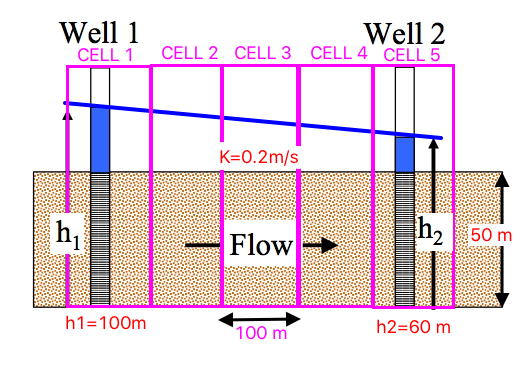
\includegraphics[width=4in]{./14-PorousMediumFlow/1D-aquifer-flow-fdm.jpg} 
   \caption{Schematic diagram of unidirectional flow in a generic aquifer, showing heads in two measuring wells.  The diagram is annotated with the cell spacing for the example (in magenta), as well as the cell ID.  The aquifer material properties are constant (K=0.2 m/s).   The head in the left well (Well 1) is 100 meters.   The head in the right well (Well 2) is 60 meters.}
   \label{fig:1D-aquifer-flow-fdm}
\end{figure}

Figure \ref{fig:1D-aquifer-flow-fdm} is the original sketch, annotated with cell spacing, material properties, and the head at the two wells.  In the figure, Well 1 has a head measurement of 100 meters, whereas Well 2 has a head measurement of 60 meters.  Because the flow is steady, and the material properties are spatially invariant, the EGL/HGL would be a line (the blue one in the figure) connecting the wells sloping from Well 1 to Well 2.

We will use the cell balance model to estimate the EGL/HGL in the aquifer (i.e. find the piezometric surface\footnote{Hydraulic head or piezometric head is a specific measurement of liquid pressure above a geodetic datum. It is usually measured as a liquid surface elevation, expressed in units of length, at the entrance (or bottom) of a piezometer. In an aquifer, it can be calculated from the depth to water in a piezometric well, and given information of the piezometer's elevation and screen depth.} between the two wells).

\begin{lstlisting}[caption=R code demonstrating an Aquifer Flow Simulator for Steady Flow \\ This fragment of code contains ..., label=lst:AquiferFlowSteady1Dimensional]
# 1D-confined-aquifer-steady-flow
# Implements Finite-Difference Porous Medium Flow using Jacobi Iteration
# Assumes boundary cells 1 and ncells are fixed head cells.
zz <- file("input1.dat", "r") # Open a connection named zz to file named input.dat
#
# read the simulation conditions
#
deltax <-as.numeric(readLines(zz, n = 1, ok = TRUE, warn = TRUE,encoding = "unknown", skipNul = FALSE))
deltay <-as.numeric(readLines(zz, n = 1, ok = TRUE, warn = TRUE,encoding = "unknown", skipNul = FALSE))
deltaz <-as.numeric(readLines(zz, n = 1, ok = TRUE, warn = TRUE,encoding = "unknown", skipNul = FALSE))
ncells <-as.numeric(readLines(zz, n = 1, ok = TRUE, warn = TRUE,encoding = "unknown", skipNul = FALSE))
tolerance <- as.numeric(readLines(zz, n = 1, ok = TRUE, warn = TRUE,encoding = "unknown", skipNul = FALSE))
hydhead <-(readLines(zz, n = 1, ok = TRUE, warn = TRUE,encoding = "unknown", skipNul = FALSE))
hydcond <-(readLines(zz, n = 1, ok = TRUE, warn = TRUE,encoding = "unknown", skipNul = FALSE))
close(zz)
#
# split the multiple column strings into numeric components for a vector
#
hydhead <-as.numeric(unlist(strsplit(hydhead,split=" ")))
hydcond <-as.numeric(unlist(strsplit(hydcond,split=" ")))
#
# built a position array for plotting
#
distance<-numeric(ncells)
distance[1]<-deltax/2.0
for (i in 2:ncells){distance[i]<-distance[i-1]+deltax}
#
# Plot Distance vs. Head before calculations
#
plot(distance,hydhead,col="red",xlim=c(0,deltax*ncells),ylim=c(0,max(hydhead)*2.0),pch=21,tck=1)
lines(distance,hydhead,col="red",type="l",lwd=3)
#
# built the transmissivity arrays
#
amat<-numeric(ncells) # make an ncells long array
bmat<-numeric(ncells) # make an ncells long array
for(irow in 2:(ncells-1)){
  amat[irow]<-((hydcond[irow-1]+hydcond[irow  ])*deltay*deltaz)/(2.0*deltax)
  bmat[irow]<-((hydcond[irow  ]+hydcond[irow+1])*deltay*deltaz)/(2.0*deltax)
}
#
# #se Jacobi iteration to find a solution to the difference equations
# 
headold<-hydhead # copy the head array, used to test for stopping 
maxit <- 100 # set the maximum number of iterations (to prevent infinite loop)
for (iter in 1:maxit){
  for (irow in 2:(ncells-1)){
    hydhead[irow]<-(amat[irow]*hydhead[irow-1]+bmat[irow]*hydhead[irow+1])/(amat[irow]+bmat[irow])
  }
# test for stopping iterations
  percentdiff <- sum((hydhead-headold)^2)
  if (percentdiff < tolerance){break}
  headold<-hydhead
}
#
# Add the steady-flow solution to the graph -- both points and a line.
#
lines(distance,hydhead,col="blue",type="p")
lines(distance,hydhead,col="blue",type="l",lwd=3)
\end{lstlisting}

Listing \ref{lst:AquiferFlowSteady1Dimensional} is a \textbf{R} script that reads an input file, computes the head distirbution (the ``blue line'') and plots the result.   The script also plots the initial values of the heads used in the computation engine.  Only the left most value and right most value remain unchanged as they represent the boundary conditions for the problem.

The iterative method is elementary for this case -- the replication of the head array at each step is used to test for stopping when the solution meets some tolerance.  The compute, test, update part of the script is a common structure in iterative problems, and when we modify the program for transient (time-varying) behavior it will come in handy.   There is no error trapping in the example -- so it is quite possible to supply an input file that would not work.  

Listing \ref{lst:1D-input-case1} is the contents of the input file (\texttt{input1.dat}) that is read by the script. 
To model different condtions, we would change the input file contents and leave the script alone.

\begin{lstlisting}[caption= Input File for Example Problem \\ This fragment of code contains ..., label=lst:1D-input-case1]
100
100
 50
5
1e-12
100 100 100 100 60
0.2 0.2 0.2 0.2 0.2
\end{lstlisting}

\begin{figure}[h!] %  figure placement: here, top, bottom, or page
   \centering
   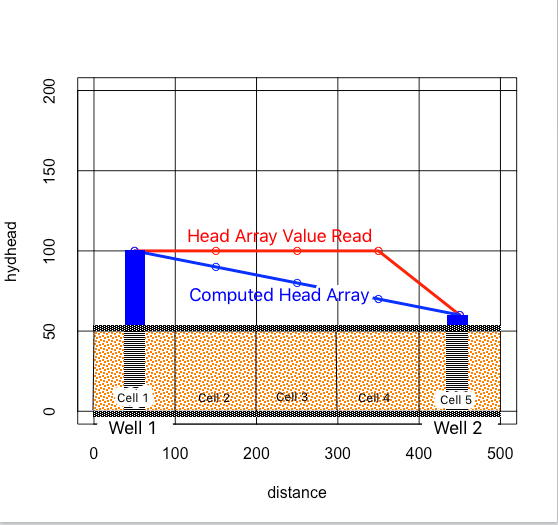
\includegraphics[width=4in]{./14-PorousMediumFlow/aquifer-1d-solution-case1.jpg} 
   \caption{Plot of computed head in each cell using Jacobi interation.   The head in the left well (Well 1) is 100 meters.   The head in the right well (Well 2) is 60 meters.  The steady flow solution is the blue line labelled ``Computed Head Array".}
   \label{fig:aquifer-1d-solution-case1}
\end{figure}
\newpage
Finally, for this problem Figure \ref{fig:aquifer-1d-solution-case1} is the output graphics from the script.  The red line is the value of heads supplied in the input file (these can be any values as long as the left and right values represent the conditions at the two wells); the blue line is the computed piezometric surface.  The markers are the computed head for each cell.

\textbf{Example 2: 1D Steady Flow in a Confined Aquifer using Gaussian Reduction}
The second example is the identical physical situation, but instead of iterative computations in our code, we will instead construct a simultaneous linear system ($Ax=b$) where the coefficient matrix $A$ is constructed from the difference equations and solved simultaneously.   

First we have to specify how to construct the matrices -- essentially because $h_1$ and $h_5$ are known, there are only three unknowns in the 5-cell example.  So we will have a linear system with 3 equations and 3 unknowns.  Here is the linear system in the context of the development of the difference equations.

\begin{displaymath}
\footnotesize
\begin{matrix}
-(A_2+B_2)\times h_2  & B_2\times h_3 & 0 \times h_4&  = & -A_3 \times h_1\\
A_3 \times h_2& -(A_3+B_3) \times h_3& B_3 \times h_4&  = & 0\\
0 \times h_2 & A_4 \times h_3 & -(A_4+B_4) \times h_4 & = & - B_4 \times h_5\\
 \end{matrix}
 \normalsize
 \end{displaymath}
 
 A more compact representation is
 \begin{displaymath}
\footnotesize
\begin{pmatrix}
-(A_2+B_2)  & B_2 & 0 \\
A_3 & -(A_3+B_3) & B_3 \\
0 & A_4 & -(A_4+B_4) \\
 \end{pmatrix}
 \begin{pmatrix}
 h_2 \\ h_3 \\ h_4 \\
 \end{pmatrix}
 =
  \begin{pmatrix}
 -A_3  h_1 \\ 0 \\ - B_4  h_5 \\
 \end{pmatrix}
 \normalsize
 \end{displaymath}
 Recall that the values for the coefficient matrix are known, as are the values $h_1$ and $h_5$.
 Now we will modify the script, to use the linear system solver and dispense with the iteration entirely.
 
 The modification(s) are to read in the values for the material and spatial properties -- just use the same code.  
 Then construct the compact matrix-vector equation by careful looping on the index values. 
 In the 5 cell example, only the inner three cells [2-4] are part of the linear system. 
 So we use indexing in the arithmetic to build the coefficient matrix and right-hand-side.
 
 Then when we have the solution, we need to put the computed values back into their correct position in the head vector.
 Listing \ref{lst:AquiferFlowSteady1DimensionalLinearSys} is a code listing that performs the various tasks.
 The script is intentionally built to use the same input file as the prior example. 
 
 The computed results are identical (as anticipated).  
 The next step (and the point of building such tools) is to try different spatial sizing (partly to be sure the code is generic and automatically adapts to such changes), and to apply the tool to aquifers with different material properties.

\clearpage 
 \begin{lstlisting}[caption= R code demonstrating an Aquifer Flow Simulator for Steady Flow  \\ 
 This version constructs coefficient matrix then solves the linear system. The program uses the same input
 file, label=lst:AquiferFlowSteady1DimensionalLinearSys]
# 1D-confined-aquifer-steady-flow
# Implements Finite-Difference Porous Medium Flow using Gaussian reduction
# Assumes boundary cells 1 and ncells are fixed head cells.
zz <- file("input1.dat", "r") # Open a connection named zz to file named input.dat
# read the simulation conditons
deltax <-as.numeric(readLines(zz, n = 1, ok = TRUE, warn = TRUE,encoding = "unknown", skipNul = FALSE))
deltay <-as.numeric(readLines(zz, n = 1, ok = TRUE, warn = TRUE,encoding = "unknown", skipNul = FALSE))
deltaz <-as.numeric(readLines(zz, n = 1, ok = TRUE, warn = TRUE,encoding = "unknown", skipNul = FALSE))
ncells <-as.numeric(readLines(zz, n = 1, ok = TRUE, warn = TRUE,encoding = "unknown", skipNul = FALSE))
tolerance <- as.numeric(readLines(zz, n = 1, ok = TRUE, warn = TRUE,encoding = "unknown", skipNul = FALSE))
hydhead <-(readLines(zz, n = 1, ok = TRUE, warn = TRUE,encoding = "unknown", skipNul = FALSE))
hydcond <-(readLines(zz, n = 1, ok = TRUE, warn = TRUE,encoding = "unknown", skipNul = FALSE))
close(zz)
# split the multiple column strings into numeric components for a vector
hydhead <-as.numeric(unlist(strsplit(hydhead,split=" ")))
hydcond <-as.numeric(unlist(strsplit(hydcond,split=" ")))

# built a position array for plotting
distance<-numeric(ncells)
distance[1]<-deltax/2.0
for (i in 2:ncells){distance[i]<-distance[i-1]+deltax}
plot(distance,hydhead,col="red",xlim=c(0,deltax*ncells),ylim=c(0,max(hydhead)*2.0),pch=21,tck=1)
lines(distance,hydhead,col="red",type="l",lwd=3)
# built the transmissivity arrays
amat<-numeric(ncells) # make an ncells long array
bmat<-numeric(ncells) # make an ncells long array
for(irow in 2:(ncells-1)){
  amat[irow]<-((hydcond[irow-1]+hydcond[irow  ])*deltay*deltaz)/(2.0*deltax)
  bmat[irow]<-((hydcond[irow  ]+hydcond[irow+1])*deltay*deltaz)/(2.0*deltax)
}
amatrix <- matrix(0,ncells-2,ncells-2)  # prefill matrix with zeros
rhs <- matrix(0,ncells-2)               # prefill vector with zeros
####################################################################
## build matrices here -- there are array indexing things going on #
## because we only have three equations to deal with.              #
## hydhead[1] is the left boundary                                 #
## hydhead[ncells] is the right boundary                           #
##  Only build the non-zero elements using the structure of the    #
##  difference-equation stencil (mask, computational molecule ...) #
####################################################################
## first row special
for (irow in 1:1){
  amatrix[irow,1]=-1.0*(amat[irow+1]+bmat[irow+1])
  amatrix[irow,2]=bmat[irow+1]
  rhs[irow] = -amat[irow+1]*hydhead[irow]
}
## interior rows
for (irow in 2:(ncells-3)){
  amatrix[irow,irow-1]=amat[irow+1] 
  amatrix[irow,irow]= -1.0*(amat[irow+1]+bmat[irow+1])
  amatrix[irow,irow+1]= bmat[irow+1]
}
## last row special
for (irow in (ncells-2):(ncells-2)){
  amatrix[irow,ncells-3]=amat[irow+1] 
  amatrix[irow,ncells-2]=-1.0*(amat[irow+1]+bmat[irow+1])
  rhs[irow] = -bmat[irow+1]*hydhead[irow+2]
}
####################################################################
## Now solve the linear system amatrix*unkvector=rhs for unkvector #
##  then put values from unkvector into correct position hydhead   #
####################################################################
unkvector<-solve(amatrix,rhs)
for (irow in 2:(ncells-1)){
  hydhead[irow] <- unkvector[irow-1]
}
###################################################################
## Plot the computed values in blue                               #
###################################################################
lines(distance,hydhead,col="blue",type="p")
lines(distance,hydhead,col="blue",type="l",lwd=3)
\end{lstlisting}
\clearpage
The next part of the example is what is the cell size is changed?  
The whole point of input files and such to to keep the script generic.  
So to check this situation, lets halve the space size (50 meters spacing, instead of 100 meters).
Thus instead of 5 cells of 100 meters each, we now have 5 cells of 50 meters each.
Listing \ref{lst:1D-input-case2} is a listing of what the input file looks like, other than twice as many initial heads and K values, essentially the same input.
\begin{lstlisting}[caption= Input File for Example Problem \\ , label=lst:1D-input-case2]
50 << changed cell size
100
 50
9 << more cells
1e-12
100 100 100 100 100 100 100 100 60 << more cells
0.2 0.2 0.2 0.2 0.2 0.2 0.2 0.2 0.2 0.2 << more cells
\end{lstlisting}

\begin{figure}[h!] %  figure placement: here, top, bottom, or page
   \centering
   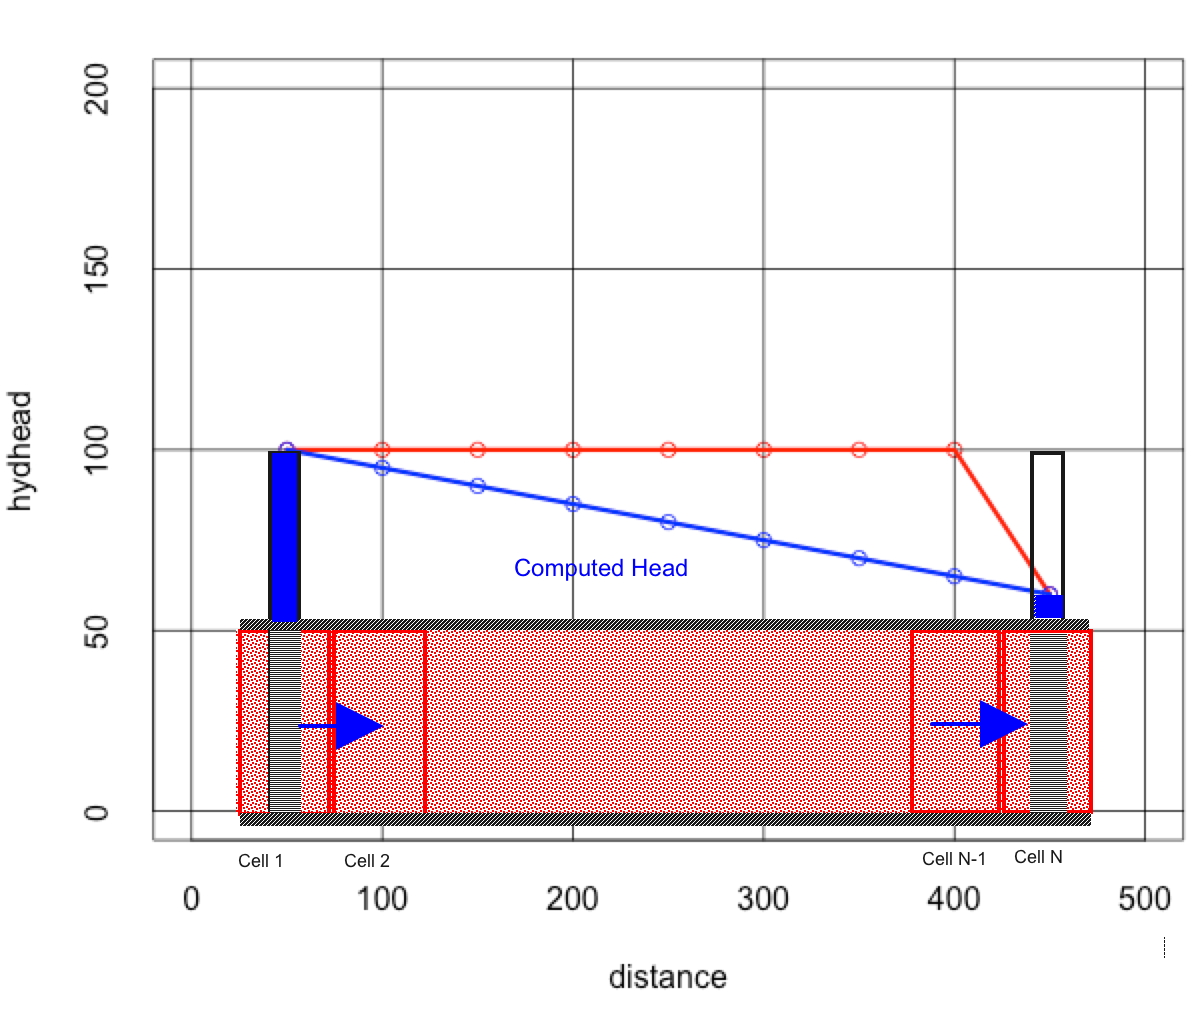
\includegraphics[width=4in]{./14-PorousMediumFlow/aquifer-1d-solution-case2.jpg} 
   \caption{Plot of computed head in each cell using different cell spacing.   The head in the left well (Well 1) is 100 meters.   The head in the right well (Well 2) is 60 meters.  The steady flow solution is the blue line labelled ``Computed Head Array".}
   \label{fig:aquifer-1d-solution-case2}
\end{figure}

Lastly, before we move to 2-Dimensional cases, lets examine when the material properties change.  
In this change, we will leave the first third of the aquifer with the same properties, but decrease hydraulic conductivity in the next third by 1/2 and the last third by 1/4 again.

Listing \ref{lst:1D-input-case3} is the input file for this case.  The anticipated result is that the HGL/EGL will change slope twice (starting out shallow, and getting steeper as we move to the right).
\clearpage
\begin{lstlisting}[caption= Input File for Example Problem \\ , label=lst:1D-input-case3]
50 
100
 50
9 << 
1e-12
100 100 100 100 100 100 100 100 60 << more cells
0.2 0.2 0.2 0.1 0.1 0.1 0.05 0.05 0.05 << more cells
\end{lstlisting}

Figure \ref{fig:aquifer-1d-solution-case3} is the results with this different input file and indeed as anticipated there are three different slopes (it looks like curvature on the plot, but its really just three different line segments with different slopes.).

\begin{figure}[h!] %  figure placement: here, top, bottom, or page
   \centering
   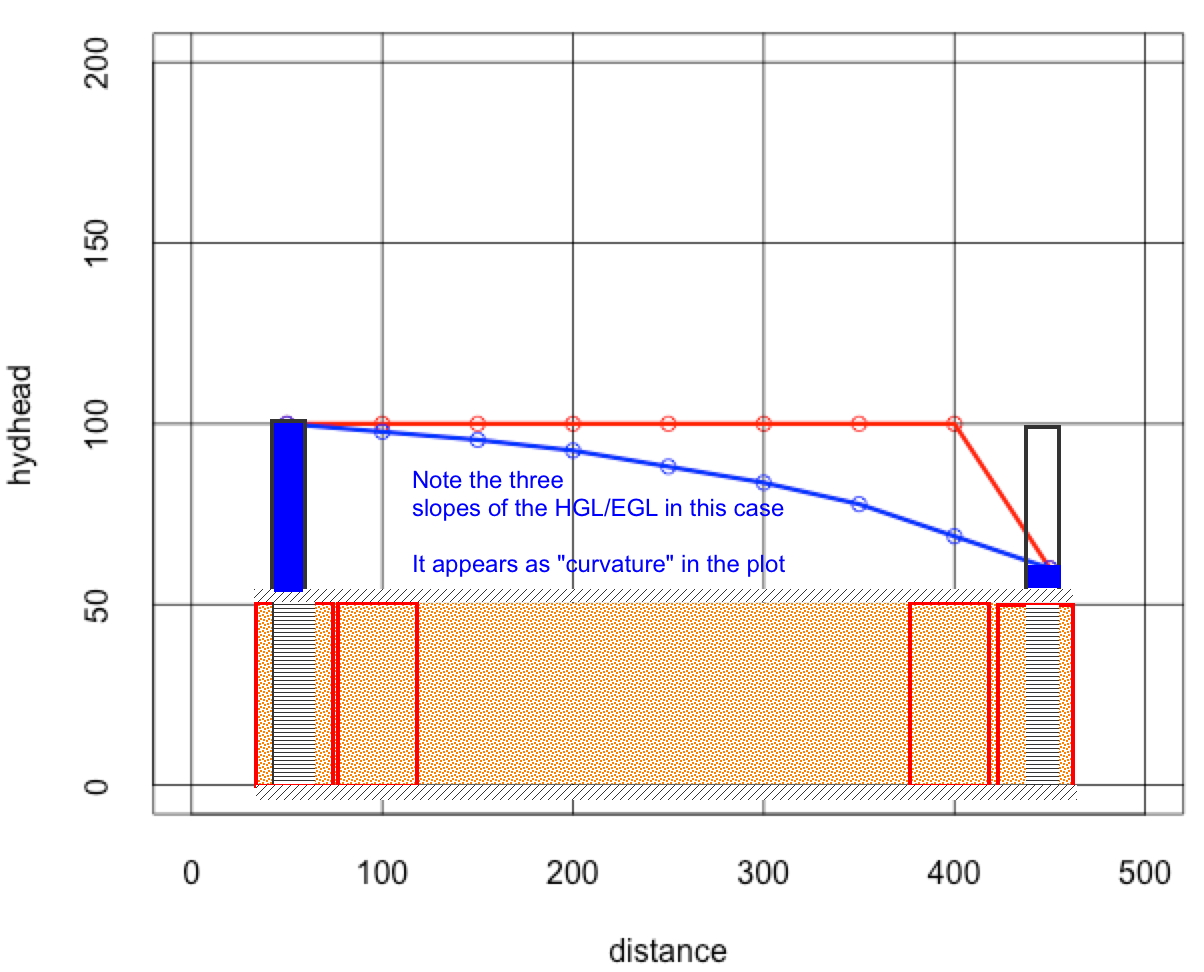
\includegraphics[width=4in]{./14-PorousMediumFlow/aquifer-1d-solution-case3.jpg} 
   \caption{Plot of computed head in each cell using different cell spacing.   The head in the left well (Well 1) is 100 meters.   The head in the right well (Well 2) is 60 meters.  The steady flow solution is the blue line.  The apparent curvature is really the three different slopes anticipated as the material properties change.}
   \label{fig:aquifer-1d-solution-case3}
\end{figure}
%%%%%%%%%%%%%%%%%%%%%%%%%%%%%%%%%%%%%%
%%%%%%%%%%%%%%%%%%%%%%%%%%%%%%%%%%%%%%
%%%%%%%%%%%%%%%%%%%%%%%%%%%%%%%%%%%%%%
\subsubsection{Finite-Difference Methods -- 2 Spatial Dimensions}
If we perform an analysis in the same way as we did to arrive at Equation \ref{eqn:finite-difference-structure} except now include another direction (the $y$-direction) we will have an aquifer in two spatial dimensions.  The governing equation becomes
  
\begin{equation}
S \frac{\partial h}{\partial t} = 
\frac{\partial}{\partial x}({T_x \frac{\partial h}{\partial x}})
+
\frac{\partial}{\partial y}({T_y \frac{\partial h}{\partial y}})
\end{equation}

The meanings of the terms are the same, except the transmissivity terms now have subscripts to indicate they can have different values depending on direction.

Then as before we will construct the difference-equation model from a multiple-cell balance model of the aquifer at a cell of interest, then extend the equations to cover the entire model domain.

Figure \ref{fig:multiple-cell-balance-2d} is a plan view schematic of a aquifer with flow to be computed in two directions ($x$ and $y$).   The cell indexing convention in the sketch is that rows are indexed by the letter $j$ and columns are indexed by the letter $i$.  This naming convention is arbitrary; in some instances it is probably preferable to reverse the convention.
The schematic also shows the assumed flow directions; for column $i$, flows are upward in the drawing, and for row $j$, flows are from left to right.  If indeed the opposite is true for a given set of boundary conditions and material properties, then the flows will be computed as negative numbers -- hence the convention here is that ``positive flow'' is right and up.  
\begin{figure}[h!] %  figure placement: here, top, bottom, or page
   \centering
   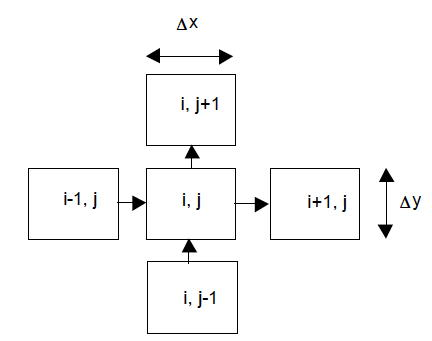
\includegraphics[width=4in]{./14-PorousMediumFlow/multiple-cell-balance-2d.jpg} 
   \caption{Plan view schematic of 2-dimensional multiple cell balance computational stencil}
   \label{fig:multiple-cell-balance-2d}
\end{figure}

As in the one-dimensional development the storage term is 
\begin{equation}
{\frac{d M_{water}}{dt}\mid}_{cell} =\rho_{w} S_{s} \Delta x \Delta y \Delta z \frac{\partial h_i}{\partial t}
\end{equation}
 where $h_i$ is the head in the $i-$th cell.  
 
 The mass flows entering the $i-\text{th},j-\text{th}$ cell are:
 \begin{equation}
M_{Inflow} = Q_{left} + Q_{bottom}=
\rho_{w} K_{x} \Delta y \Delta z \frac{h_{i-1,j} - h_{i,j}}{\Delta x} +
\rho_{w} K_{y} \Delta x \Delta z \frac{h_{i,j-1} - h_{i,j}}{\Delta y}                  
\end{equation}
 
The mass flows leaving the $i-\text{th},j-\text{th}$ cell are:
\begin{equation}
M_{Inflow} = Q_{right} + Q_{top}=
\rho_{w} K_{x} \Delta y \Delta z \frac{h_{i,j} - h_{i+1,j}}{\Delta x} +
\rho_{w} K_{y} \Delta x \Delta z \frac{h_{i,j} - h_{i,j+1}}{\Delta y}                  
\end{equation}

Now write the entire balance equation

\begin{equation}
\begin{matrix}
\rho_{w} S_{s} \Delta x \Delta y \Delta z \frac{\partial h_i}{\partial t} = 
[\rho_{w} K_{x} \Delta y \Delta z \frac{h_{i-1,j} - h_{i,j}}{\Delta x} +
\rho_{w} K_{y} \Delta x \Delta z \frac{h_{i,j-1} - h_{i,j}}{\Delta y}] - \\
~~~~~~~~~~\\
~~~~~~~~~~[\rho_{w} K_{x} \Delta y \Delta z \frac{h_{i,j} - h_{i+1,j}}{\Delta x} +
\rho_{w} K_{y} \Delta x \Delta z \frac{h_{i,j} - h_{i,j+1}}{\Delta y} ]        
\end{matrix}        
\end{equation}

Next replace $S_s \Delta z$ with the storage coefficient $S$, and the $K_{x,y} \Delta z$ with the transmissivity $T_{x,y}$ terms, and divide by the density of the fluid and the cell plan view area $\Delta x \Delta y$ to obtain a more compact form of the difference equation.

\begin{equation}
\begin{matrix}
S \frac{\partial h_i}{\partial t} = 
[\frac{1}{\Delta x} T_{x} \frac{h_{i-1,j} - h_{i,j}}{\Delta x} +
 \frac{1}{\Delta y} T_{y} \frac{h_{i,j-1} - h_{i,j}}{\Delta y}] - \\
~~~~~~~~~~\\
~~~~~~~~~~[ \frac{1}{\Delta x} T_{x}  \frac{h_{i,j} - h_{i+1,j}}{\Delta x} +
  \frac{1}{\Delta y}  T_{y} \frac{h_{i,j} - h_{i,j+1}}{\Delta y} ]        
\end{matrix}        
\end{equation}

As in the one-dimensional case, lets again consider steady flow (we will do transient flows later on)

\begin{equation}
\begin{matrix}
0= 
[\frac{1}{\Delta x} T_{x} \frac{h_{i-1,j} - h_{i,j}}{\Delta x} +
 \frac{1}{\Delta y} T_{y} \frac{h_{i,j-1} - h_{i,j}}{\Delta y}] - \\
~~~~~~~~~~\\
~~~~~~~~~~[ \frac{1}{\Delta x} T_{x}  \frac{h_{i,j} - h_{i+1,j}}{\Delta x} +
  \frac{1}{\Delta y}  T_{y} \frac{h_{i,j} - h_{i,j+1}}{\Delta y} ]        
\end{matrix}        
\end{equation}

Also as in the one-dimensional case, we will approximate the spatial variation of the material properties (transmissivity) as arithmetic mean values between two cells, so making the following definitions:

\begin{equation}
\begin{matrix}
A_{i,j} = \frac{1}{2 \Delta x^2}(T_{x,(i-1,j)}+T_{x,(i,j)}) \\ ~~ \\
B_{i,j} = \frac{1}{2 \Delta x^2}(T_{x,(i,j)}+T_{x,(i+1,j)})   \\ ~~ \\
C_{i,j} = \frac{1}{2 \Delta y^2}(T_{y,(i,j-1)}+T_{y,(i,j)})   \\ ~~ \\
D_{i,j} = \frac{1}{2 \Delta y^2}(T_{y,(i,j)}+T_{y,(i,j+1)})   \\ ~~ \\
\end{matrix}
\end{equation}

Substitution into the difference equation yields

\begin{equation}
0 = A_{i,j}h_{i-1,j} + B_{i,j}h_{i+1,j} - (A_{i,j}+B_{i,j}+C_{i,j}+D_{i,j})h_{i,j} + C_{i,j}h_{i,j-1} + D_{i,j}h_{i,j+1}
\end{equation}

As before we can explicitly write the cell equation for $h_{i,j}$ as

\begin{equation}
h_{i,j} = \frac{[A_{i,j}h_{i-1,j} + B_{i,j}h_{i+1,j} + C_{i,j}h_{i,j-1} + D_{i,j}h_{i,j+1}]}{[A_{i,j}+B_{i,j}+C_{i,j}+D_{i,j}]}
\end{equation}

This difference equation represents an approximation to the governing flow equation, the accuracy depending on the cell
size. Boundary conditions are applied directly into the analogs (another name for the difference equations) at appropriate
locations on the computational grid. Also as in the one-dimensional case we can generate solutions either by iteration or solving the resulting linear system.  

\textbf{Example 1: 2D Steady Flow in a Confined Aquifer using Jacobi Iteration}
As before we will start the example with a simple physical condition and use Jacobi iteration\footnote{Jacobi iteration for large domain problems (say 200x200) or bigger, is pretty inefficient -- better iterative methods are available; however they represent clever changes to the basic iteration methods explained here, hence Jacobi is a good place to start.} to obtain a solution.  
We will also incorporate two kinds of boundary conditions (fixed head as before, and no-flow boundaries).

Figure \ref{fig:aquifer-2d-layout} is a schematic of this example.   The right panel of the figure shows the index naming convention.  The known material properties are transmissivity (in each direction, at each cell center, and the thickness of the aquifer ($b == \Delta z$).
\begin{figure}[h!] %  figure placement: here, top, bottom, or page
   \centering
   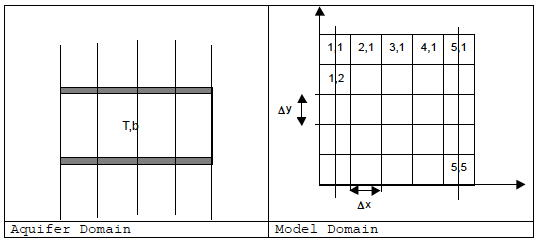
\includegraphics[width=6in]{./14-PorousMediumFlow/aquifer-2d-layout.jpg} 
   \caption{Schematic of 2-dimensional aquifer.  The left and right boundaries are constant head boundaries, whereas the upper and lower boundaries are no-flow}
   \label{fig:aquifer-2d-layout}
\end{figure}
Our task is to simulate the aquifer with the 5 x 5 model shown. 
The left and right boundaries will be treated as specified head boundaries. 
The upper and lower boundary will be treated as no flow boundaries.

The head on the left is 100 meters and the right is 60 meters (same as before).
The transmissivity ($K_{x,y} \Delta z$=10) square meters per second (but to be consistent with the earlier models we will supply a value of $K$ and $\Delta z$; keeping with the earlier examples the values are $K=0.2$ meters per second, and $\Delta z=50$ meters.
The spatial dimensions are $\Delta x = 100$ meters and $\Delta y = 100$ meters.

Listing \ref{lst:2D-Jacobi} is a listing that implements the method -- in this case there are changes to the data reading (to read and build matrices), and notice how the no-flow boundary conditions are implemented.   
\begin{lstlisting}[caption= R code demonstrating an Aquifer Flow Simulator for 2D Steady Flow.  This code fragment implements the Jacobi iteration.  A subsequent listing shows the contour plot syntax.  In the example the two fragments are joined and run as a single source file \\ , label=lst:2D-Jacobi]
# Implements 2D-Confined Aquifer Steady Flow Finite-Difference using Jacobi Iteration
# Assumes no-flow boundary row=1,and nrows.  Assumes fixed head boundary col=1, and ncols
# Head boundary conditions are entered in input file
zz <- file("input1.dat", "r") # Open a connection named zz to file named input.dat
# read the simulation conditons
deltax <-as.numeric(readLines(zz, n = 1, ok = TRUE, warn = TRUE,encoding = "unknown", skipNul = FALSE))
deltay <-as.numeric(readLines(zz, n = 1, ok = TRUE, warn = TRUE,encoding = "unknown", skipNul = FALSE))
deltaz <-as.numeric(readLines(zz, n = 1, ok = TRUE, warn = TRUE,encoding = "unknown", skipNul = FALSE))
nrows <-as.numeric(readLines(zz, n = 1, ok = TRUE, warn = TRUE,encoding = "unknown", skipNul = FALSE))
ncols <-as.numeric(readLines(zz, n = 1, ok = TRUE, warn = TRUE,encoding = "unknown", skipNul = FALSE))
tolerance <- as.numeric(readLines(zz, n = 1, ok = TRUE, warn = TRUE,encoding = "unknown", skipNul = FALSE))
hydhead <-(readLines(zz, n = nrows, ok = TRUE, warn = TRUE,encoding = "unknown", skipNul = FALSE))
hydcondx <-(readLines(zz, n = nrows, ok = TRUE, warn = TRUE,encoding = "unknown", skipNul = FALSE))
hydcondy <-(readLines(zz, n = nrows, ok = TRUE, warn = TRUE,encoding = "unknown", skipNul = FALSE))
close(zz)
# split the multiple column strings into numeric components for a vector
hydhead <-as.numeric(unlist(strsplit(hydhead,split=" ")))
hydcondx <-as.numeric(unlist(strsplit(hydcondx,split=" ")))
hydcondy <-as.numeric(unlist(strsplit(hydcondy,split=" ")))
# convert the numeric vectors into matrices for easier indexing
hydhead <-matrix(hydhead,nrow=nrows,ncol=ncols,byrow = TRUE)
hydcondx <-matrix(hydcondx,nrow=nrows,ncol=ncols,byrow = TRUE)
hydcondy <-matrix(hydcondy,nrow=nrows,ncol=ncols,byrow = TRUE)
# built the transmissivity arrays
amat<-matrix(0,nrows,ncols) 
bmat<-matrix(0,nrows,ncols) 
cmat<-matrix(0,nrows,ncols)
dmat<-matrix(0,nrows,ncols)
for(irow in 2:(nrows-1)){
  for(jcol in 2:(ncols-1)){
amat[irow,jcol]<-((hydcondx[irow-1,jcol  ]+hydcondx[irow  ,jcol  ])*deltaz)/(2.0*deltax^2)
bmat[irow,jcol]<-((hydcondx[irow  ,jcol  ]+hydcondx[irow+1,jcol  ])*deltaz)/(2.0*deltax^2)
cmat[irow,jcol]<-((hydcondy[irow  ,jcol-1]+hydcondy[irow  ,jcol  ])*deltaz)/(2.0*deltay^2)
dmat[irow,jcol]<-((hydcondy[irow  ,jcol  ]+hydcondy[irow  ,jcol+1])*deltaz)/(2.0*deltay^2)
  }
}
headold<-hydhead # copy the head array, used to test for stopping 
maxit <- 100 # set the maximum number of iterations (to prevent infinite loop)
for (iter in 1:maxit){
  # first and last row special == no flow boundaries
  for(jcol in 1:ncols){
    hydhead[1,jcol]=hydhead[2,jcol]
    hydhead[nrows,jcol]=hydhead[nrows-1,jcol]
  }
  for (irow in 2:(nrows-1)){
    for (jcol in 2:(nrows-1)){
      hydhead[irow,jcol] = 
        (amat[irow,jcol]*hydhead[irow-1,jcol  ] +
         bmat[irow,jcol]*hydhead[irow+1,jcol  ] +
         cmat[irow,jcol]*hydhead[irow  ,jcol-1] +
         dmat[irow,jcol]*hydhead[irow  ,jcol+1]  )/
        (amat[irow,jcol]+bmat[irow,jcol]+cmat[irow,jcol]+dmat[irow,jcol])
    }
  }
# test for stopping iterations
  percentdiff <- sum((hydhead-headold)^2)
  if (percentdiff < tolerance){
    message("Exit iterations because tolerance met")
    break}
  headold<-hydhead  #update the current head vector
}\end{lstlisting}
\clearpage

Instead of line plots, the built-in contouring algorithm in \textbf{R} is used to render the output plot(s).  Listing \ref{lst:2D-Contour} is the script that generates a contour plot.  The rows are actually plotted in the vertical, and columns in the horizontal, so the plot is rotated relative to the definition sketch.\footnote{This kind of plotting is a hold-over from line-printer days, where the long axis would be oriented to the vertical so that it could print to its heart's content and still fit on the paper. Older tractor-feed line-printers could print 135 characters wide, and as long as the paper roll held out.  The paper was called green-bar; each perforated sheet was 11x17 and the sheets were connected.  Essentially the paper length was functionally infinite, but the width was fixes at 17 inches.}

\begin{lstlisting}[caption= R code demonstrating building a contour plot from the computed head distribution \\ , label=lst:2D-Contour]
##############################################################
###    built position arrays for contour plotting          ###
##############################################################
distancex<-numeric(nrows)
distancey<-numeric(ncols)
distancex[1]<-50
distancey[1]<-50
for (irow in 2:nrows){distancex[irow]<-distancex[irow-1]+deltax}
for (jcol in 2:ncols){distancey[jcol]<-distancey[jcol-1]+deltay}
##############################################################
###    contour plot of head -- note axes are rotated       ###
##############################################################
contour(distancex,distancey,hydhead,
        plot.title = title(main = "Steady 2D Aquifer Model (Head in Meters)",
                           xlab = "Meters (Y axis) ====>>", 
                           ylab = "Meters (X axis) ====>>"))
\end{lstlisting}

Listing \ref{lst:2D-input-case1} is a listing of the input file.  The only major change from the one-dimensional examples is the entire head and transmissivity arrays are supplied.  

\begin{lstlisting}[caption= Input File for Example Problem \\ , label=lst:2D-input-case1]
100
100
 50
5
5
1e-12
100 100 100 100 60
100 100 100 100 60
100 100 100 100 60
100 100 100 100 60
100 100 100 100 60
0.2 0.2 0.2 0.2 0.2
0.2 0.2 0.2 0.2 0.2
0.2 0.2 0.2 0.2 0.2
0.2 0.2 0.2 0.2 0.2
0.2 0.2 0.2 0.2 0.2
\end{lstlisting}

\begin{figure}[h!] %  figure placement: here, top, bottom, or page
   \centering
   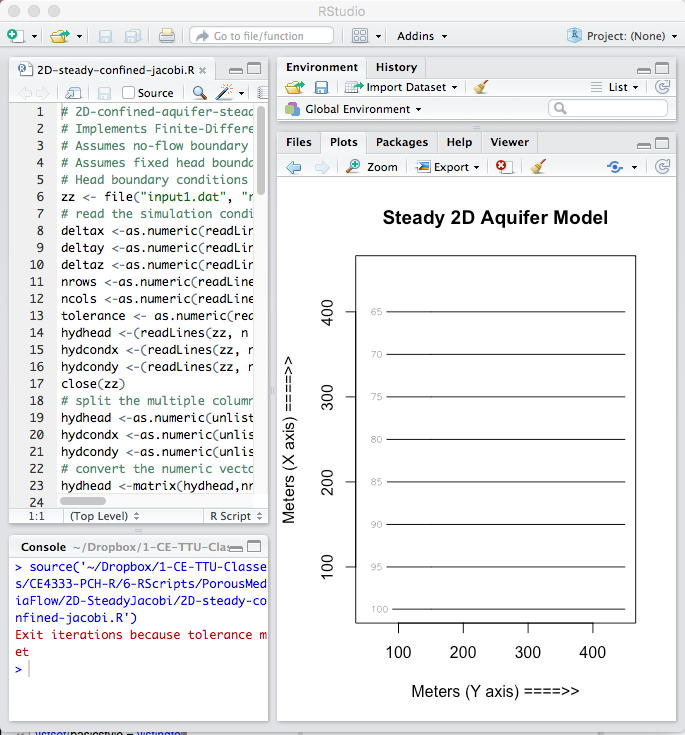
\includegraphics[height=6in]{./14-PorousMediumFlow/aquifer-2d-contour1.jpg} 
   \caption{Output from \textbf{R} script for 2D model.  Observe how the X-axis is plotted upward, and the Y-axis is plotter left to right.  The plotting is because of how ROWS and COLUMNS were indexed in the script.  Rather than alter the script, I find it easier to rotate the problem for practical application.}
   \label{fig:aquifer-2d-contour1}
\end{figure}
Figure \ref{fig:aquifer-2d-contour1} is a screen capture of the \textbf{R} output (using the R studio IDE).   The plot is on the right side of the screen image.
Figure \ref{fig:aquifer-2d-contour2} is a screen capture of just the plot, rotated, and with the boundaries identified (no-flow top and bottom; fixed head left and right).

\begin{figure}[h!] %  figure placement: here, top, bottom, or page
   \centering
   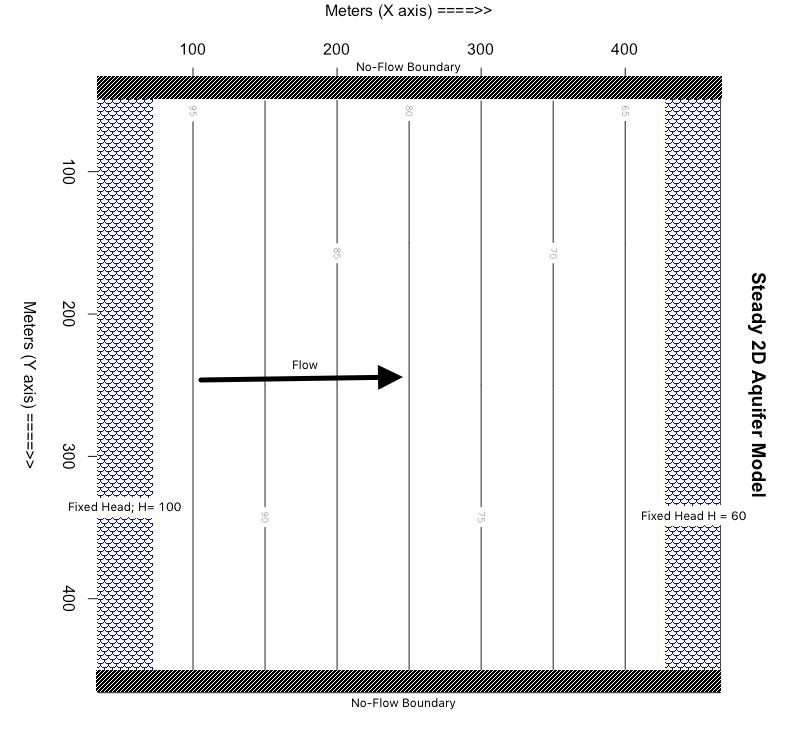
\includegraphics[height=6in]{./14-PorousMediumFlow/aquifer-2d-contour2.jpg} 
   \caption{Output from \textbf{R} script for 2D model, rotated and annotated to fit the original problem statement}
   \label{fig:aquifer-2d-contour2}
\end{figure}

Inspection of the script shows that there are still some parts of the script that could use generalization (namely the graphics portion, and a more sophisticated approach to boundary conditions), but otherwise we have the beginnings of a useful tool.   

\textbf{Example 3: 2D Stream Function using Jacobi Iteration}
In steady aquifer flow, the flow is irrotational (or at least can be modeled as such). 
There exists an orthogonal function called the stream function (it is the function that exists in the flow field when vorticity is zero).
A really good explaination of stream functions (and streamlines) appears on pages 381--398 in \cite{Zheng1995}.

This function can be used to generate plots of streamlines for the same system.
The principal changes are the material properties representation and the boundary conditions.  

The stream function $\Psi$ as a partial differential equation is
\begin{equation}
0= 
\frac{\partial}{\partial x}({\frac{1}{T_y} \frac{\partial \Psi}{\partial x}})
+
\frac{\partial}{\partial y}({\frac{1}{T_x} \frac{\partial \Psi}{\partial y}})
\end{equation}

Observe how the material property is inverted and changes directional identity, otherwise the equation is structurally identical to the groundwater flow equation (for steady flow).

The difference equation is also almost the same

\begin{equation}
\begin{matrix}
0= 
[\frac{1}{\Delta x} \frac{1}{T_{y}} \frac{\Psi_{i-1,j} - \Psi_{i,j}}{\Delta x} +
 \frac{1}{\Delta y} \frac{1}{T_{x}} \frac{\Psi_{i,j-1} - \Psi_{i,j}}{\Delta y}] - \\
~~~~~~~~~~\\
~~~~~~~~~~[ \frac{1}{\Delta x} \frac{1}{T_{y}}  \frac{\Psi_{i,j} - \Psi_{i+1,j}}{\Delta x} +
  \frac{1}{\Delta y}  \frac{1}{T_{x}} \frac{\Psi_{i,j} - \Psi_{i,j+1}}{\Delta y} ]        
\end{matrix}        
\end{equation}

The substitutions are

\begin{equation}
\begin{matrix}
A_{i,j} = \frac{1}{2 \Delta x^2}(T_{y,(i-1,j)}^{-1}+T_{y,(i,j)}^{-1}) \\ ~~ \\
B_{i,j} = \frac{1}{2 \Delta x^2}(T_{y,(i,j)}^{-1}+T_{y,(i+1,j)}^{-1})   \\ ~~ \\
C_{i,j} = \frac{1}{2 \Delta y^2}(T_{x,(i,j-1)}^{-1}+T_{x,(i,j)}^{-1})   \\ ~~ \\
D_{i,j} = \frac{1}{2 \Delta y^2}(T_{x,(i,j)}^{-1}+T_{x,(i,j+1)}^{-1})   \\ ~~ \\
\end{matrix}
\end{equation}

Substitution into the difference equation yields

\begin{equation}
0 = A_{i,j}\Psi_{i-1,j} + B_{i,j}\Psi_{i+1,j} - (A_{i,j}+B_{i,j}+C_{i,j}+D_{i,j})\Psi_{i,j} + C_{i,j}\Psi_{i,j-1} + D_{i,j}\Psi_{i,j+1}
\end{equation}

As before we can explicitly write the cell equation for $h_{i,j}$ as

\begin{equation}
\Psi_{i,j} = \frac{[A_{i,j}\Psi_{i-1,j} + B_{i,j}\Psi_{i+1,j} + C_{i,j}\Psi_{i,j-1} + D_{i,j}\Psi_{i,j+1}]}{[A_{i,j}+B_{i,j}+C_{i,j}+D_{i,j}]}
\end{equation}

So at this point we could literally use the same script, however boundary conditions also ``invert.''
A no-flow head-domain boundary is a constant value stream function-domain boundary.
A constant value head-domain boundary is a zero-gradient stream function-domain boundary.

So we could use the same code, but probably are better off building a separate code (it can read the same input file), and use it to generate stream functions.  
The prior example code is modified to generate the stream function for its case (and plot the stream function contours), which if overlaid on the head contours produces a flow net.
%After the example is presented, the two contour plots will be overlaid outside of \textbf{R}.\footnote{I will be using macOS programs to render the two plots into a single plot.  
%What the analyst has to do is to make both plots and save them.  Then choose one plot, and render all ``white pixels" as transparent.  Then take this new image and import onto the other plot.  The result is a flownet for the aquifer system.} 

The modified code literally changes the names of the head array to stream function, modifies how the material properties ($A,B,C,D$) are constructed, and modified how the boundary conditions are incorporated.  Listing \ref{lst:2D-JacobiStream} is a listing that implements the method -- notice how the no-flow boundary conditions are implemented.   

In this example the value of the stream function is arbitrarily set to range from $0$ to $100$.  One useful interpretation of stream function values is that their differences indicate the flow fraction (of total flow) that flows between the streamlines (contour lines of constant stream function value).
\clearpage

\begin{lstlisting}[caption= R code demonstrating an Stream Function Simulator for 2D Steady Flow.  This code fragment implements the Jacobi iteration.  A subsequent listing shows the contour plot syntax.  In the example the two fragments are joined and run as a single source file \\ , label=lst:2D-JacobiStream]
# 2D-streamfunction
# Implements Finite-Difference Stream Function using Jacobi Iteration
# Assumes no-flow boundary row=1,and nrows ==> constant stream function
# Assumes fixed head boundary col=1, and ncols ==> no-flux stream function -- stream function runs from 0 to 100
zz <- file("input1.dat", "r") # Open a connection named zz to file named input.dat
# read the simulation conditons
deltax <-as.numeric(readLines(zz, n = 1, ok = TRUE, warn = TRUE,encoding = "unknown", skipNul = FALSE))
deltay <-as.numeric(readLines(zz, n = 1, ok = TRUE, warn = TRUE,encoding = "unknown", skipNul = FALSE))
deltaz <-as.numeric(readLines(zz, n = 1, ok = TRUE, warn = TRUE,encoding = "unknown", skipNul = FALSE))
nrows <-as.numeric(readLines(zz, n = 1, ok = TRUE, warn = TRUE,encoding = "unknown", skipNul = FALSE))
ncols <-as.numeric(readLines(zz, n = 1, ok = TRUE, warn = TRUE,encoding = "unknown", skipNul = FALSE))
tolerance <- as.numeric(readLines(zz, n = 1, ok = TRUE, warn = TRUE,encoding = "unknown", skipNul = FALSE))
streamfn <-(readLines(zz, n = nrows, ok = TRUE, warn = TRUE,encoding = "unknown", skipNul = FALSE))
hydcondx <-(readLines(zz, n = nrows, ok = TRUE, warn = TRUE,encoding = "unknown", skipNul = FALSE))
hydcondy <-(readLines(zz, n = nrows, ok = TRUE, warn = TRUE,encoding = "unknown", skipNul = FALSE))
close(zz)
# split the multiple column strings into numeric components for a vector
streamfn <-as.numeric(unlist(strsplit(streamfn,split=" ")))
hydcondx <-as.numeric(unlist(strsplit(hydcondx,split=" ")))
hydcondy <-as.numeric(unlist(strsplit(hydcondy,split=" ")))
# convert the numeric vectors into matrices for easier indexing
streamfn <-matrix(streamfn,nrow=nrows,ncol=ncols,byrow = TRUE)
hydcondx <-matrix(hydcondx,nrow=nrows,ncol=ncols,byrow = TRUE)
hydcondy <-matrix(hydcondy,nrow=nrows,ncol=ncols,byrow = TRUE)
# built the transmissivity arrays
amat<-matrix(0,nrows,ncols) 
bmat<-matrix(0,nrows,ncols) 
cmat<-matrix(0,nrows,ncols)
dmat<-matrix(0,nrows,ncols)
for(irow in 2:(nrows-1)){
  for(jcol in 2:(ncols-1)){
    amat[irow,jcol]<-((1.0/hydcondy[irow-1,jcol  ]+1.0/hydcondy[irow  ,jcol  ])*deltaz)/(2.0*deltax^2)
    bmat[irow,jcol]<-((1.0/hydcondy[irow  ,jcol  ]+1.0/hydcondy[irow+1,jcol  ])*deltaz)/(2.0*deltax^2)
    cmat[irow,jcol]<-((1.0/hydcondx[irow  ,jcol-1]+1.0/hydcondx[irow  ,jcol  ])*deltaz)/(2.0*deltay^2)
    dmat[irow,jcol]<-((1.0/hydcondx[irow  ,jcol  ]+1.0/hydcondx[irow  ,jcol+1])*deltaz)/(2.0*deltay^2)
  }
}
# begin the calculations
streamold<-streamfn # copy the head array, used to test for stopping 
maxit <- 100 # set the maximum number of iterations (to prevent infinite loop)
for (iter in 1:maxit){
  # first and last row special == no flow boundaries in head, fixed value streamfunction
  for(jcol in 1:ncols){
    streamfn[1,jcol]=0.0
    streamfn[nrows,jcol]=100.0
  }
  for (irow in 2:(nrows-1)){
  # first and last columns special == fixed head boundaries, no-gradient stream function
    streamfn[irow,1]=streamfn[irow,2]
    streamfn[irow,nrows]=streamfn[irow,nrows-1]
    for (jcol in 2:(nrows-1)){
      streamfn[irow,jcol] = 
        (amat[irow,jcol]*streamfn[irow-1,jcol  ] +
         bmat[irow,jcol]*streamfn[irow+1,jcol  ] +
         cmat[irow,jcol]*streamfn[irow  ,jcol-1] +
         dmat[irow,jcol]*streamfn[irow  ,jcol+1]  )/
        (amat[irow,jcol]+bmat[irow,jcol]+cmat[irow,jcol]+dmat[irow,jcol])
    }
  }
# test for stopping iterations
  percentdiff <- sum((streamfn-streamold)^2)
  if (percentdiff < tolerance){
    message("Exit iterations because tolerance met")
    break}
  streamold<-streamfn  #update the current head vector
}
}\end{lstlisting}
\clearpage

\begin{lstlisting}[caption= R code demonstrating an Stream Function Simulator for 2D Steady Flow.  This code fragment implements the contour plotting \\ , label=lst:2D-ContourStream]
# echo contents for debugging
# streamfn
# streamold
##############################################################
###    built position arrays for contour plotting          ###
##############################################################
distancex<-numeric(nrows)
distancey<-numeric(ncols)
distancex[1]<-50
distancey[1]<-50
for (irow in 2:nrows){distancex[irow]<-distancex[irow-1]+deltax}
for (jcol in 2:ncols){distancey[jcol]<-distancey[jcol-1]+deltay}
##############################################################
###    contour plot of head -- note axes are rotated       ###
##############################################################
contour(distancex,distancey,streamfn,
        plot.title = title(main = "Stream Function Model",
                           xlab = "Meters (Y axis) ====>>", 
                           ylab = "Meters (X axis) ====>>"))
}\end{lstlisting}

Figure \ref{fig:streamfn-2d-contour1} is the stream function result.  
Compare it to Figure \ref{fig:aquifer-2d-contour1} and it should be clear that the ``lines'' are at right angles to each other --that is the stream function is orthogonal to the head function (which is anticipated, because of the nature of the relationship between stream function and head functions; the orthogonality is a consequence of the flow satisfying the the Cauchy-Riemann conditions.).

\begin{figure}[h!] %  figure placement: here, top, bottom, or page
   \centering
   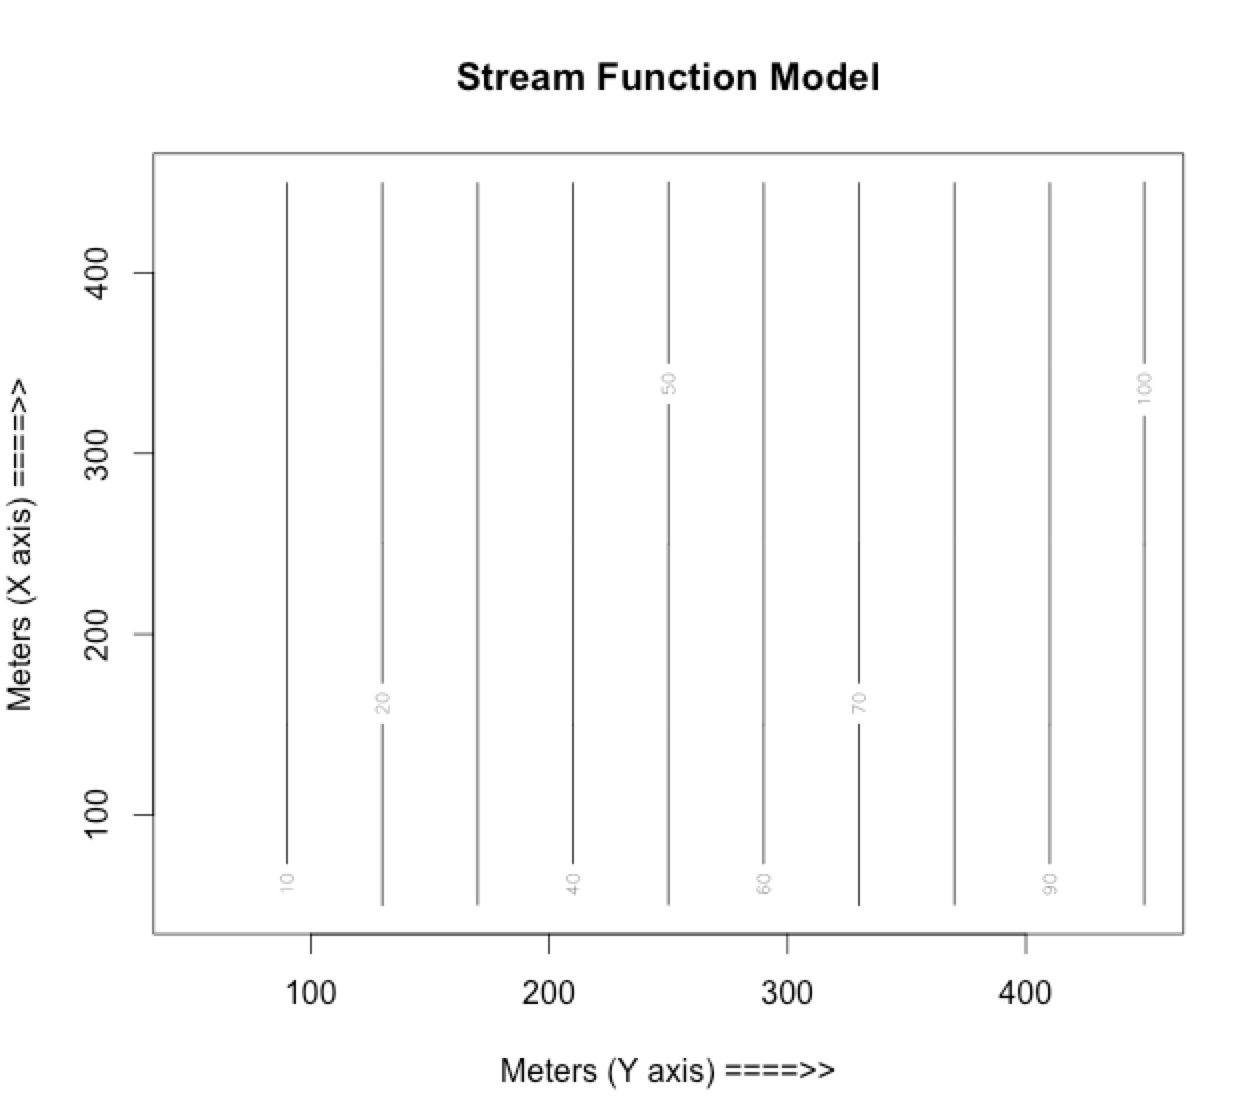
\includegraphics[height=4in]{./14-PorousMediumFlow/streamfn-2d-contour1.jpg} 
   \caption{Output from \textbf{R} script for stream function model.}
   \label{fig:streamfn-2d-contour1}
\end{figure}

To complete the example, and prepare for the next example, we will modify the script one more time to:
\begin{enumerate}
\item Read in the material property values, head values, etc.  (no change).
\item Compute the head distribution.
\item Compute the stream function distribution. (merge the two scripts)
\item Plot the head and stream function on the same graph -- use different colors.  Also rotate the plots so axes agree with the problem statement.
\end{enumerate}

Figure \ref{fig:streamfn-2d-contour2} is the result of these modifications.  


\begin{figure}[h!] %  figure placement: here, top, bottom, or page
   \centering
   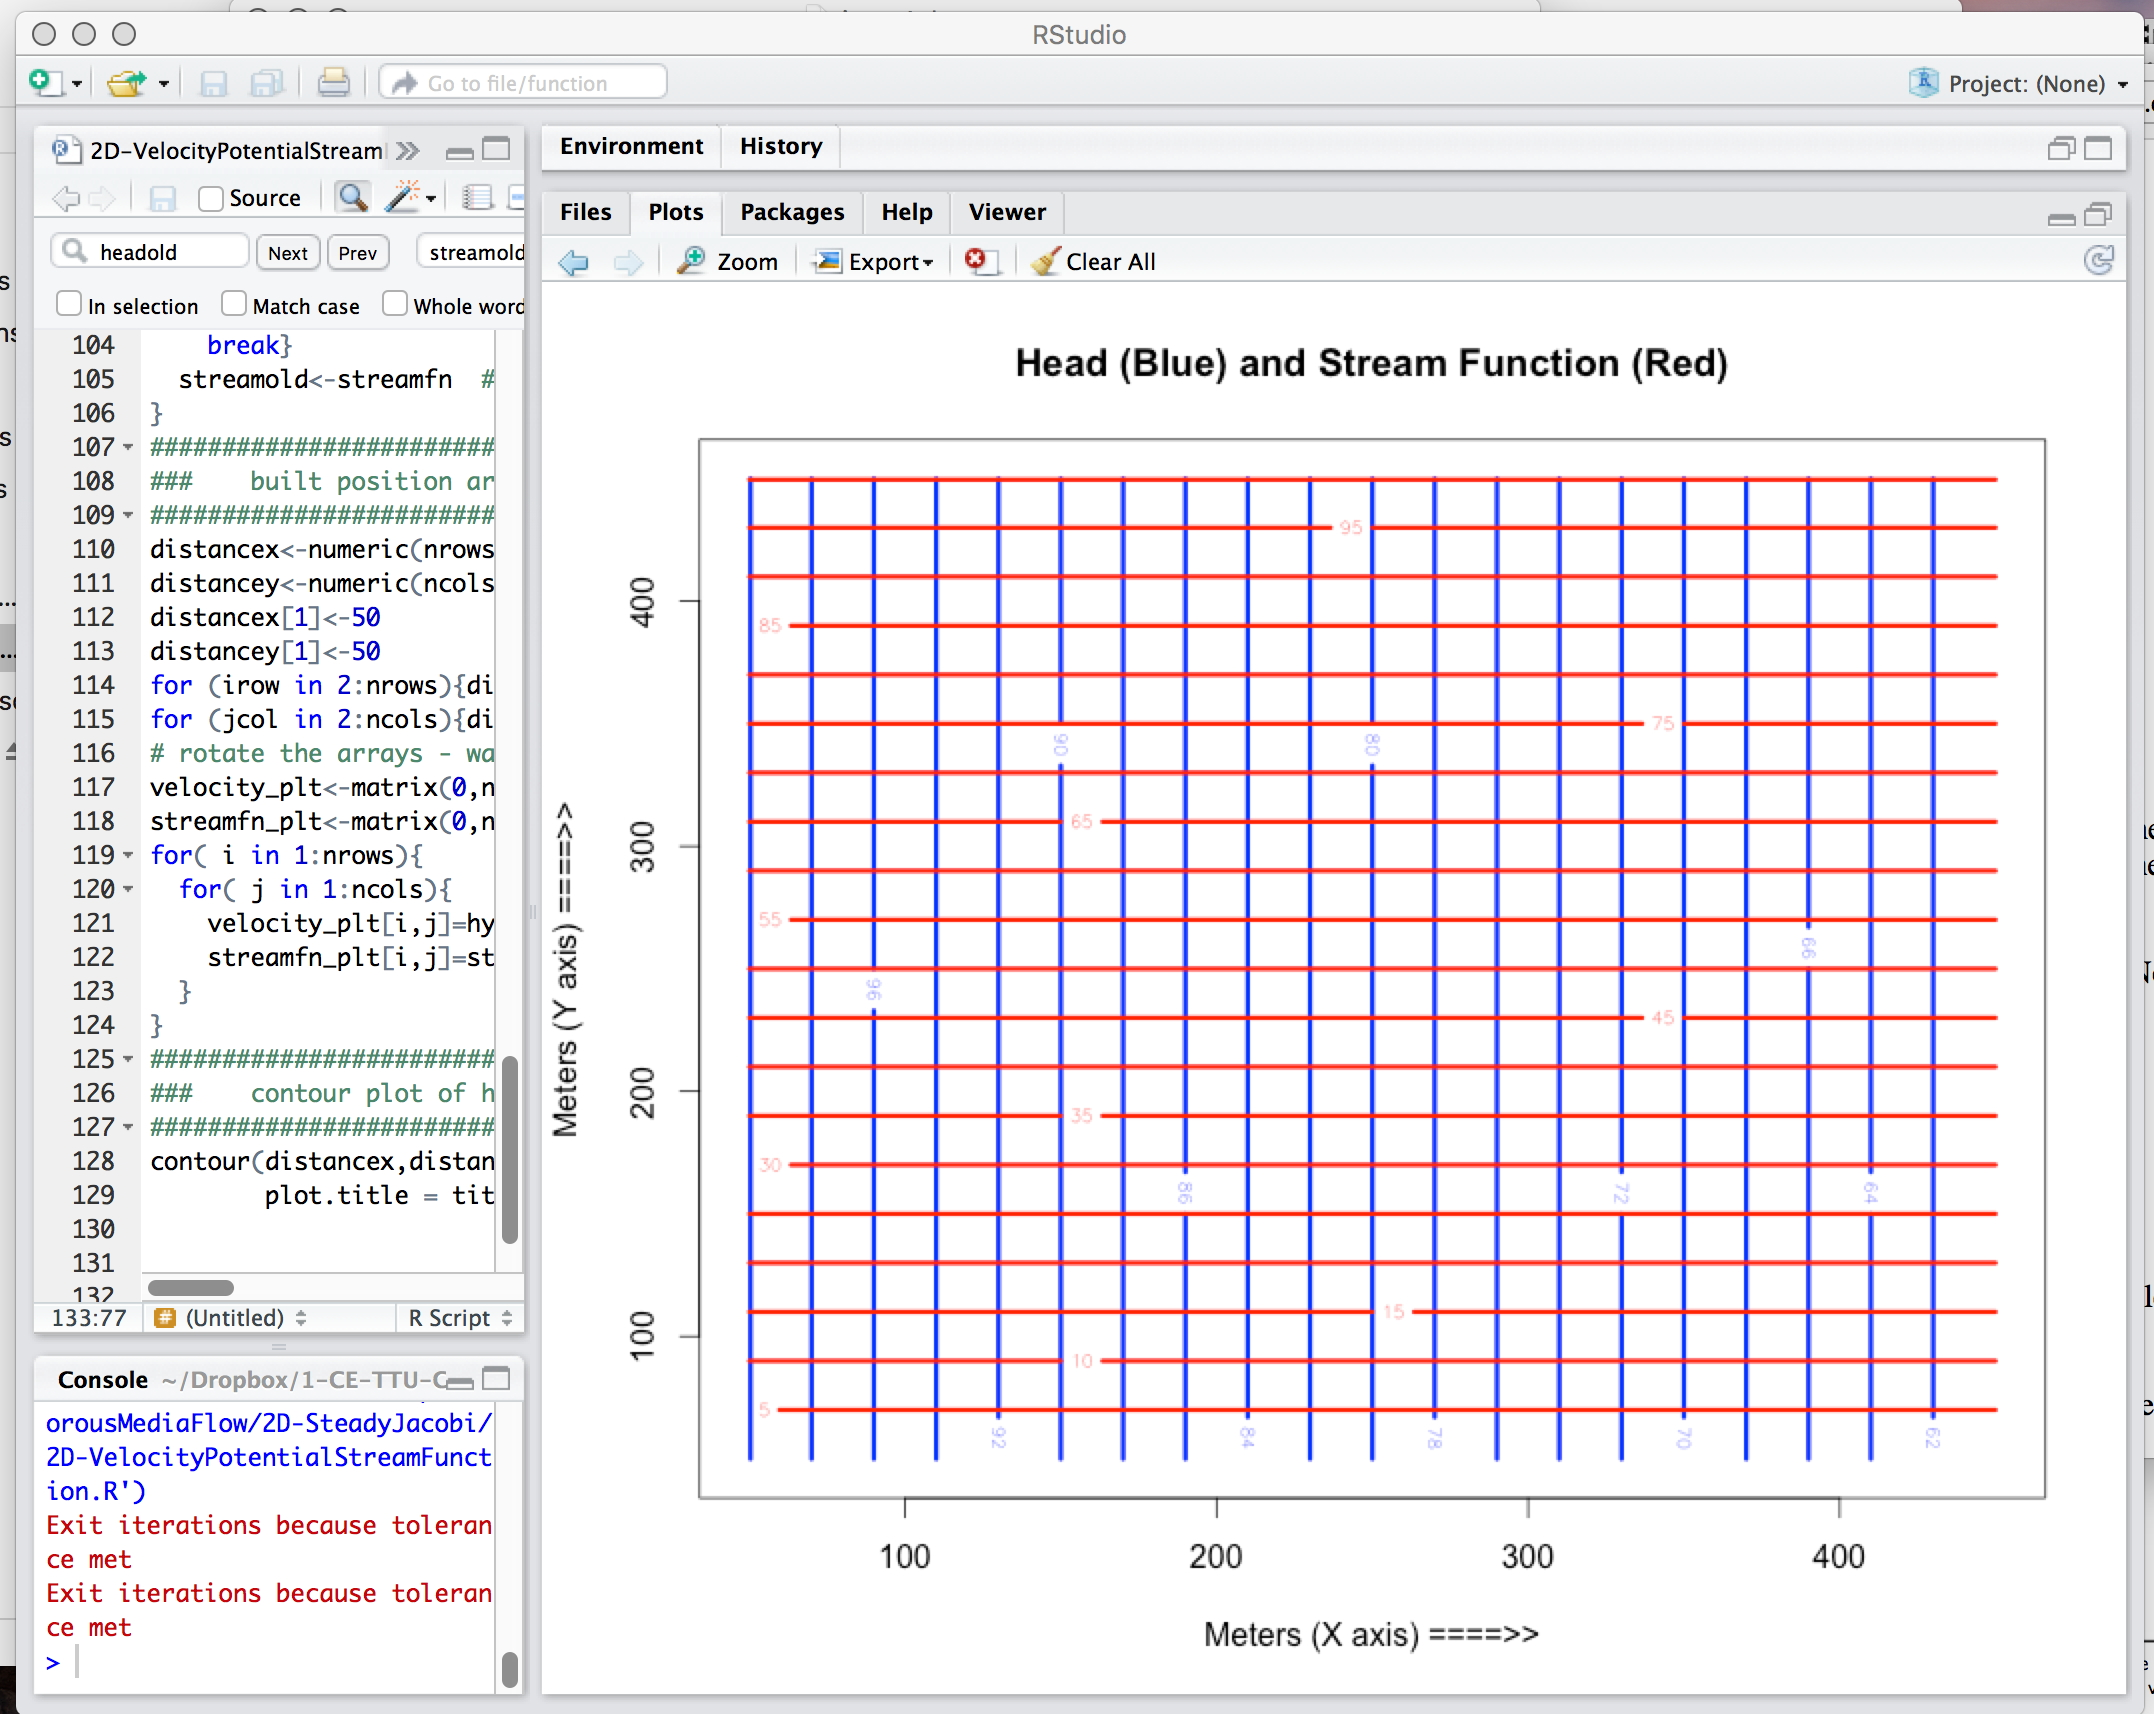
\includegraphics[height=4.5in]{./14-PorousMediumFlow/streamfn-2d-contour2.jpg} 
   \caption{Output from \textbf{R} script for velocity-potential, stream function model, rotated and annotated to fit the original problem statement}
   \label{fig:streamfn-2d-contour2}
\end{figure}

Listing \ref{lst:velocitypotential} is a script fragment that implements the velocity-potential (here the same thing as the head equations) portion of the computations.  
The data file is the same, the only difference is the head values are copied to another vector (the stream functions) for use in the next fragment.

Listing \ref{lst:streamfunction} is a script fragment that implements the stream-function calculations.  
The $A,B,C,D$ matrices are re-initialized and re-used.
The stream function values are computed using the same computation engine (code is repeated --  generally poor practice; done here to illustrate the re-use).

Listing \ref{lst:2by2contour} is the script fragment that rotates the results and plots the flow net.
\clearpage

\begin{lstlisting}[caption= R code demonstrating an Velocity Potential (Aquifer Head) Simulator for 2D Steady Flow.  This code fragment implements the contour plotting \\ , label=lst:velocitypotential]
# 2D Velocity Potential Stream Function Model
# hydhead is velocity potential
# streamfm is stream function
zz <- file("input1.dat", "r") # Open a connection named zz to file named input.dat
# read the simulation conditons
deltax <-as.numeric(readLines(zz, n = 1, ok = TRUE, warn = TRUE,encoding = "unknown", skipNul = FALSE))
deltay <-as.numeric(readLines(zz, n = 1, ok = TRUE, warn = TRUE,encoding = "unknown", skipNul = FALSE))
deltaz <-as.numeric(readLines(zz, n = 1, ok = TRUE, warn = TRUE,encoding = "unknown", skipNul = FALSE))
nrows <-as.numeric(readLines(zz, n = 1, ok = TRUE, warn = TRUE,encoding = "unknown", skipNul = FALSE))
ncols <-as.numeric(readLines(zz, n = 1, ok = TRUE, warn = TRUE,encoding = "unknown", skipNul = FALSE))
tolerance <- as.numeric(readLines(zz, n = 1, ok = TRUE, warn = TRUE,encoding = "unknown", skipNul = FALSE))
hydhead <-(readLines(zz, n = nrows, ok = TRUE, warn = TRUE,encoding = "unknown", skipNul = FALSE))
hydcondx <-(readLines(zz, n = nrows, ok = TRUE, warn = TRUE,encoding = "unknown", skipNul = FALSE))
hydcondy <-(readLines(zz, n = nrows, ok = TRUE, warn = TRUE,encoding = "unknown", skipNul = FALSE))
close(zz)
# split the multiple column strings into numeric components for a vector
hydhead <-as.numeric(unlist(strsplit(hydhead,split=" ")))
hydcondx <-as.numeric(unlist(strsplit(hydcondx,split=" ")))
hydcondy <-as.numeric(unlist(strsplit(hydcondy,split=" ")))
# convert the numeric vectors into matrices for easier indexing
hydhead <-matrix(hydhead,nrow=nrows,ncol=ncols,byrow = TRUE)
hydcondx <-matrix(hydcondx,nrow=nrows,ncol=ncols,byrow = TRUE)
hydcondy <-matrix(hydcondy,nrow=nrows,ncol=ncols,byrow = TRUE)
# copy the hydhead array into streamfn for later use
streamfn <- hydhead
# here we perform the velocity potential calculations
# built the transmissivity arrays
amat<-matrix(0,nrows,ncols) 
bmat<-matrix(0,nrows,ncols) 
cmat<-matrix(0,nrows,ncols)
dmat<-matrix(0,nrows,ncols)
for(irow in 2:(nrows-1)){
  for(jcol in 2:(ncols-1)){
    amat[irow,jcol]<-((hydcondx[irow-1,jcol  ]+hydcondx[irow  ,jcol  ])*deltaz)/(2.0*deltax^2)
    bmat[irow,jcol]<-((hydcondx[irow  ,jcol  ]+hydcondx[irow+1,jcol  ])*deltaz)/(2.0*deltax^2)
    cmat[irow,jcol]<-((hydcondy[irow  ,jcol-1]+hydcondy[irow  ,jcol  ])*deltaz)/(2.0*deltay^2)
    dmat[irow,jcol]<-((hydcondy[irow  ,jcol  ]+hydcondy[irow  ,jcol+1])*deltaz)/(2.0*deltay^2)
  }
}
# veloity potential
headold<-hydhead # copy the head array, used to test for stopping 
maxit <- 100 # set the maximum number of iterations (to prevent infinite loop)
for (iter in 1:maxit){
  # first and last row special == no flow boundaries
  for(jcol in 1:ncols){
    hydhead[1,jcol]=hydhead[2,jcol]
    hydhead[nrows,jcol]=hydhead[nrows-1,jcol]
  }
  for (irow in 2:(nrows-1)){
    for (jcol in 2:(nrows-1)){
      hydhead[irow,jcol] = 
        (amat[irow,jcol]*hydhead[irow-1,jcol  ] +
           bmat[irow,jcol]*hydhead[irow+1,jcol  ] +
           cmat[irow,jcol]*hydhead[irow  ,jcol-1] +
           dmat[irow,jcol]*hydhead[irow  ,jcol+1]  )/
        (amat[irow,jcol]+bmat[irow,jcol]+cmat[irow,jcol]+dmat[irow,jcol])
    }
  }
  # test for stopping iterations
  percentdiff <- sum((hydhead-headold)^2)
  if (percentdiff < tolerance){
    message("Exit iterations because tolerance met")
    break}
  headold<-hydhead  #update the current head vector
}
}\end{lstlisting}
\clearpage

\begin{lstlisting}[caption= R code demonstrating an Stream Function Simulator for 2D Steady Flow.  This code fragment implements the stream function \\ , label=lst:streamfunction]
# built the streamfn transmissivity arrays  -- notice reuse of the a,b,c,d arrays
amat<-matrix(0,nrows,ncols) 
bmat<-matrix(0,nrows,ncols) 
cmat<-matrix(0,nrows,ncols)
dmat<-matrix(0,nrows,ncols)
for(irow in 2:(nrows-1)){
  for(jcol in 2:(ncols-1)){
    amat[irow,jcol]<-((1.0/hydcondy[irow-1,jcol  ]+1.0/hydcondy[irow  ,jcol  ])*deltaz)/(2.0*deltax^2)
    bmat[irow,jcol]<-((1.0/hydcondy[irow  ,jcol  ]+1.0/hydcondy[irow+1,jcol  ])*deltaz)/(2.0*deltax^2)
    cmat[irow,jcol]<-((1.0/hydcondx[irow  ,jcol-1]+1.0/hydcondx[irow  ,jcol  ])*deltaz)/(2.0*deltay^2)
    dmat[irow,jcol]<-((1.0/hydcondx[irow  ,jcol  ]+1.0/hydcondx[irow  ,jcol+1])*deltaz)/(2.0*deltay^2)
  }
}
streamold<-streamfn # copy the head array, used to test for stopping 
maxit <- 100 # set the maximum number of iterations (to prevent infinite loop)
for (iter in 1:maxit){
  # first and last row special == no flow boundaries in head, fixed value streamfunction
  for(jcol in 1:ncols){
    streamfn[1,jcol]=0.0
    streamfn[nrows,jcol]=100.0
  }
  for (irow in 2:(nrows-1)){
  # first and last columns special == fixed head boundaries, no-gradient stream function
    streamfn[irow,1]=streamfn[irow,2]
    streamfn[irow,nrows]=streamfn[irow,nrows-1]
    for (jcol in 2:(nrows-1)){
      streamfn[irow,jcol] = 
        (amat[irow,jcol]*streamfn[irow-1,jcol  ] +
         bmat[irow,jcol]*streamfn[irow+1,jcol  ] +
         cmat[irow,jcol]*streamfn[irow  ,jcol-1] +
         dmat[irow,jcol]*streamfn[irow  ,jcol+1]  )/
        (amat[irow,jcol]+bmat[irow,jcol]+cmat[irow,jcol]+dmat[irow,jcol])
    }
  }
# test for stopping iterations
  percentdiff <- sum((streamfn-streamold)^2)
  if (percentdiff < tolerance){
    message("Exit iterations because tolerance met")
    break}
  streamold<-streamfn  #update the current head vector
}
}\end{lstlisting}
\clearpage

\begin{lstlisting}[caption= R code demonstrating an Velocity Potential -- Stream Function Simulator for 2D Steady Flow.  This code fragment implements the contour plotting \\ , label=lst:2by2contour]
##############################################################
###    built position arrays for contour plotting          ###
##############################################################
distancex<-numeric(nrows)
distancey<-numeric(ncols)
distancex[1]<-50
distancey[1]<-50
for (irow in 2:nrows){distancex[irow]<-distancex[irow-1]+deltax}
for (jcol in 2:ncols){distancey[jcol]<-distancey[jcol-1]+deltay}
# rotate the arrays - wasting memory.  Fix for homework.
velocity_plt<-matrix(0,nrows,ncols) 
streamfn_plt<-matrix(0,nrows,ncols) 
for( i in 1:nrows){
  for( j in 1:ncols){
    velocity_plt[i,j]=hydhead[j,i]
    streamfn_plt[i,j]=streamfn[j,i]
  }
}
##############################################################
###    contour plot of head -- note axes are rotated       ###
##############################################################
contour(distancex,distancey,velocity_plt,
        plot.title = title(main = "Head (Blue) and Stream Function (Red)",
                           xlab = "Meters (X axis) ====>>", 
                           ylab = "Meters (Y axis) ====>>"),
        col="blue",lwd=3,xlim=c(50,450),ylim=c(50,450),nlevels=20)
contour(distancey,distancex,streamfn_plt,add=TRUE,col="red",lwd=3,nlevels=20)
}\end{lstlisting}

\clearpage
\textbf{Example 3: 2D Flow Net in a Confined Aquifer using Jacobi Iteration with Low Permeability Inclusion}

Figure \ref{fig:aquifer-2d-lowKinclusion} is a schematic of a different situation that now only requires us to change the contents of the data file, and re-run the scripts unchanged.  
Some additional modifications have been added, mostly messages to the user because of anticipated long run times.    
The data file is changed a bit and two lines are added to help with the plotting -- they represent the axis labels used in the contour plots.
The boundary conditions are still directly coded into the algorithm, and that would be the next modification to the code - general boundary condition information.\footnote{That modification is left for homework.}

\begin{figure}[h!] %  figure placement: here, top, bottom, or page
   \centering
   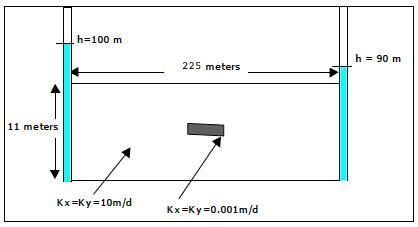
\includegraphics[width=4.5in]{./14-PorousMediumFlow/aquifer-2d-lowKinclusion.jpg} 
   \caption{Schematic of vertical slice in an aquifer with low permeability inclusion.  Values are indicated on the schematic.  Example illustrates how to use the scripts to generate flow nets for the vertical slice }
   \label{fig:aquifer-2d-lowKinclusion}
\end{figure}

The following pages contain the code fragments (listings) for the velocity potential, the stream function, and the contour plotting.  As above, these listings are combined into a single file (the fragmentation herein is to fit the printed page layout) and then run as a script. 

Listing \ref{lst:2DinclusionVelocity} is the listing for the velocity potential calculations.

Listing \ref{lst:2DinclusionStream} is the listing for the stream function calculations.

Listing \ref{lst:2DinclusionPlot} is the is the listing for the plotting calculations.

Listing \ref{lst:2DinclusionInput} is the input file for the problem.  The file in this case is named \texttt{input2.dat}.  
In addition the generalized boundary conditons, the reader should consider making the program prompt the user for the file name, so that the program is somewhat deployable.

\clearpage

\begin{lstlisting}[caption= Velocity Potential Script , label=lst:2DinclusionVelocity]
# 2D Velocity Potential Stream Function Model
# hydhead is velocity potential; streamfm is stream function
rm(list=ls())  # deallocate (clear) memory
zz <- file("input2.dat", "r") # Open a connection named zz to file named input.dat to read input conditions
deltax <-as.numeric(readLines(zz, n = 1, ok = TRUE, warn = TRUE,encoding = "unknown", skipNul = FALSE))
deltay <-as.numeric(readLines(zz, n = 1, ok = TRUE, warn = TRUE,encoding = "unknown", skipNul = FALSE))
deltaz <-as.numeric(readLines(zz, n = 1, ok = TRUE, warn = TRUE,encoding = "unknown", skipNul = FALSE))
nrows <-as.numeric(readLines(zz, n = 1, ok = TRUE, warn = TRUE,encoding = "unknown", skipNul = FALSE))
ncols <-as.numeric(readLines(zz, n = 1, ok = TRUE, warn = TRUE,encoding = "unknown", skipNul = FALSE))
tolerance <- as.numeric(readLines(zz, n = 1, ok = TRUE, warn = TRUE,encoding = "unknown", skipNul = FALSE))
distancex <- (readLines(zz, n = 1, ok = TRUE, warn = TRUE,encoding = "unknown", skipNul = FALSE))
distancey <- (readLines(zz, n = 1, ok = TRUE, warn = TRUE,encoding = "unknown", skipNul = FALSE))
hydhead <-(readLines(zz, n = nrows, ok = TRUE, warn = TRUE,encoding = "unknown", skipNul = FALSE))
hydcondx <-(readLines(zz, n = nrows, ok = TRUE, warn = TRUE,encoding = "unknown", skipNul = FALSE))
hydcondy <-(readLines(zz, n = nrows, ok = TRUE, warn = TRUE,encoding = "unknown", skipNul = FALSE))
close(zz)
# split the multiple column strings into numeric components for a vector
distancex <-as.numeric(unlist(strsplit(distancex,split=" ")))
distancey <-as.numeric(unlist(strsplit(distancey,split=" ")))
hydhead <-as.numeric(unlist(strsplit(hydhead,split=" ")))
hydcondx <-as.numeric(unlist(strsplit(hydcondx,split=" ")))
hydcondy <-as.numeric(unlist(strsplit(hydcondy,split=" ")))
# convert the numeric vectors into matrices for easier indexing
hydhead <-matrix(hydhead,nrow=nrows,ncol=ncols,byrow = TRUE)
hydcondx <-matrix(hydcondx,nrow=nrows,ncol=ncols,byrow = TRUE)
hydcondy <-matrix(hydcondy,nrow=nrows,ncol=ncols,byrow = TRUE)
# built the transmissivity arrays
amat<-matrix(0,nrows,ncols) 
bmat<-matrix(0,nrows,ncols) 
cmat<-matrix(0,nrows,ncols)
dmat<-matrix(0,nrows,ncols)
for(irow in 2:(nrows-1)){
  for(jcol in 2:(ncols-1)){
    amat[irow,jcol]<-((hydcondx[irow-1,jcol  ]+hydcondx[irow  ,jcol  ])*deltaz)/(2.0*deltax^2)
    bmat[irow,jcol]<-((hydcondx[irow  ,jcol  ]+hydcondx[irow+1,jcol  ])*deltaz)/(2.0*deltax^2)
    cmat[irow,jcol]<-((hydcondy[irow  ,jcol-1]+hydcondy[irow  ,jcol  ])*deltaz)/(2.0*deltay^2)
    dmat[irow,jcol]<-((hydcondy[irow  ,jcol  ]+hydcondy[irow  ,jcol+1])*deltaz)/(2.0*deltay^2)
  }
}
headold<-hydhead      # copy the head array, used to test for stopping 
tolflag<-FALSE
maxit <- 500000 # set the maximum number of iterations (to prevent infinite loop)
for (iter in 1:maxit){
  # first and last row special == no flow boundaries
  for(jcol in 1:ncols){
    hydhead[1,jcol]<-hydhead[2,jcol]
    hydhead[nrows,jcol]<-hydhead[nrows-1,jcol]
  }
  for (irow in 2:(nrows-1)){
    for (jcol in 2:(ncols-1)){
      hydhead[irow,jcol] <- 
        (amat[irow,jcol]*hydhead[irow-1,jcol  ] +
           bmat[irow,jcol]*hydhead[irow+1,jcol  ] +
           cmat[irow,jcol]*hydhead[irow  ,jcol-1] +
           dmat[irow,jcol]*hydhead[irow  ,jcol+1]  )/
        (amat[irow,jcol]+bmat[irow,jcol]+cmat[irow,jcol]+dmat[irow,jcol])
    }
  }
  # test for stopping iterations
  percentdiff <- sum((hydhead-headold)^2)
  if (percentdiff < tolerance){
    message("Exit iterations in velocity potential because tolerance met");
    message("Iterations =", iter);
    tolflag <- TRUE
    break}
 headold<-hydhead  #update the current head vector
 if( iter %% 5000 == 0){message("Calculating in Potential Function ",iter," of ",maxit, "iterations")}
}
if (tolflag == FALSE){message("Exit iterations in potential function at max iterations")}
}\end{lstlisting}








\begin{lstlisting}[caption= Stream Function Script , label=lst:2DinclusionStream]
streamfn<-matrix(1.0,nrows,ncols)
for (i in 1:nrows){
  for(j in 1:ncols){
    streamfn[i,j]=as.numeric(i)/as.numeric(nrows)
  }
}
streamfn
# built the streamfn transmissivity arrays
amats<-matrix(0,nrows,ncols) 
bmats<-matrix(0,nrows,ncols) 
cmats<-matrix(0,nrows,ncols)
dmats<-matrix(0,nrows,ncols)
for(irow in 2:(nrows-1)){
  for(jcol in 2:(ncols-1)){
    amats[irow,jcol]<-((1.0/hydcondy[irow-1,jcol  ]+1.0/hydcondy[irow  ,jcol  ])*deltaz)/(2.0*deltax^2)
    bmats[irow,jcol]<-((1.0/hydcondy[irow  ,jcol  ]+1.0/hydcondy[irow+1,jcol  ])*deltaz)/(2.0*deltax^2)
    cmats[irow,jcol]<-((1.0/hydcondx[irow  ,jcol-1]+1.0/hydcondx[irow  ,jcol  ])*deltaz)/(2.0*deltay^2)
    dmats[irow,jcol]<-((1.0/hydcondx[irow  ,jcol  ]+1.0/hydcondx[irow  ,jcol+1])*deltaz)/(2.0*deltay^2)
  }
}
streamold<-streamfn # copy the head array, used to test for stopping 
tolflag<-FALSE
maxit <- maxit/10 # set the maximum number of iterations (to prevent infinite loop)
for (iter in 1:maxit){
  # first and last row special == no flow boundaries in head, fixed value streamfunction
  for(jcol in 1:ncols){
    streamfn[1,jcol]=0.0
    streamfn[nrows,jcol]=1.0
  }
  for (irow in 2:(nrows-1)){
    # first and last columns special == fixed head boundaries, no-gradient stream function
    streamfn[irow,1]=streamfn[irow,2]
    streamfn[irow,ncols]=streamfn[irow,ncols-1]
    for (jcol in 2:(ncols-1)){
      streamfn[irow,jcol] = 
        (amats[irow,jcol]*streamfn[irow-1,jcol  ] +
           bmats[irow,jcol]*streamfn[irow+1,jcol  ] +
           cmats[irow,jcol]*streamfn[irow  ,jcol-1] +
           dmats[irow,jcol]*streamfn[irow  ,jcol+1]  )/
        (amats[irow,jcol]+bmats[irow,jcol]+cmats[irow,jcol]+dmats[irow,jcol])
    }
  }
  # test for stopping iterations
  percentdiff <- sum((streamfn-streamold)^2)
  if (percentdiff < tolerance)
    {
    message("Exit iterations in stream function because tolerance met");
    message("Iterations =", iter);
    tolflag <- TRUE;
    break
    }
  streamold<-streamfn  #update the current head vector
  if( iter %% 5000 == 0){message("Calculating in Stream Function ",iter," of ",maxit, "iterations")}
}
if (tolflag == FALSE){message("Exit iterations in stream function at max iterations")}
}\end{lstlisting}















\begin{lstlisting}[caption= Contour plotting script , label=lst:2DinclusionPlot]
###############################################################################
###    rotate arrays for contour plotting -- position values read in input  ###
###############################################################################
velocity_plt<-matrix(0,ncols,nrows) 
streamfn_plt<-matrix(0,ncols,nrows) 
for( i in 1:nrows){
  for( j in 1:ncols){
    velocity_plt[j,i]=hydhead[i,j]
    streamfn_plt[j,i]=streamfn[i,j]
  }
}
##############################################################
###    contour plot of head -- note axes are rotated       ###
##############################################################
contour(distancey,distancex,velocity_plt,
        plot.title = title(main = "Head (Blue) and Stream Function (Red)",
                           xlab = "Meters (X axis) ====>>", 
                           ylab = "Meters (Y axis) ====>>"),
        col="blue",lwd=3,nlevels=20)
contour(distancey,distancex,streamfn_plt,add=TRUE,col="red",lwd=3,nlevels=20)
}\end{lstlisting}

\begin{lstlisting}[caption= Input file for 2D vertical slice confined aquifer with low permeability inclusion , label=lst:2DinclusionInput]
1
10
1
13
23
1e-16
0.5 1.5 2.5 3.5 4.5 5.5 6.5 7.5 8.5 9.5 10.5 11.5 12.5
5 15 25 35 45 55 65 75 85 95 105 115 125 135 145 155 165 175 185 195 205 215 225
100 100 100 100 100 100 100 100 100 100 100 100 100 100 100 100 100 100 100 100 100 100 90
100 100 100 100 100 100 100 100 100 100 100 100 100 100 100 100 100 100 100 100 100 100 90
100 100 100 100 100 100 100 100 100 100 100 100 100 100 100 100 100 100 100 100 100 100 90
100 100 100 100 100 100 100 100 100 100 100 100 100 100 100 100 100 100 100 100 100 100 90
100 100 100 100 100 100 100 100 100 100 100 100 100 100 100 100 100 100 100 100 100 100 90
100 100 100 100 100 100 100 100 100 100 100 100 100 100 100 100 100 100 100 100 100 100 90
100 100 100 100 100 100 100 100 100 100 100 100 100 100 100 100 100 100 100 100 100 100 90
100 100 100 100 100 100 100 100 100 100 100 100 100 100 100 100 100 100 100 100 100 100 90
100 100 100 100 100 100 100 100 100 100 100 100 100 100 100 100 100 100 100 100 100 100 90
100 100 100 100 100 100 100 100 100 100 100 100 100 100 100 100 100 100 100 100 100 100 90
100 100 100 100 100 100 100 100 100 100 100 100 100 100 100 100 100 100 100 100 100 100 90
100 100 100 100 100 100 100 100 100 100 100 100 100 100 100 100 100 100 100 100 100 100 90
100 100 100 100 100 100 100 100 100 100 100 100 100 100 100 100 100 100 100 100 100 100 90
10 10 10 10 10 10 10 10 10 10 10 10 10 10 10 10 10 10 10 10 10 10 10
10 10 10 10 10 10 10 10 10 10 10 10 10 10 10 10 10 10 10 10 10 10 10
10 10 10 10 10 10 10 10 10 10 10 10 10 10 10 10 10 10 10 10 10 10 10
10 10 10 10 10 10 10 10 10 10 10 10 10 10 10 10 10 10 10 10 10 10 10
10 10 10 10 10 10 10 10 10 10 10 10 10 10 10 10 10 10 10 10 10 10 10
10 10 10 10 10 10 10 10 10 10 0.0001 0.0001 0.0001 10 10 10 10 10 10 10 10 10 10
10 10 10 10 10 10 10 10 10 10 0.0001 0.0001 0.0001 10 10 10 10 10 10 10 10 10 10
10 10 10 10 10 10 10 10 10 10 0.0001 0.0001 0.0001 10 10 10 10 10 10 10 10 10 10
10 10 10 10 10 10 10 10 10 10 10 10 10 10 10 10 10 10 10 10 10 10 10
10 10 10 10 10 10 10 10 10 10 10 10 10 10 10 10 10 10 10 10 10 10 10
10 10 10 10 10 10 10 10 10 10 10 10 10 10 10 10 10 10 10 10 10 10 10
10 10 10 10 10 10 10 10 10 10 10 10 10 10 10 10 10 10 10 10 10 10 10
10 10 10 10 10 10 10 10 10 10 10 10 10 10 10 10 10 10 10 10 10 10 10
10 10 10 10 10 10 10 10 10 10 10 10 10 10 10 10 10 10 10 10 10 10 10
10 10 10 10 10 10 10 10 10 10 10 10 10 10 10 10 10 10 10 10 10 10 10
10 10 10 10 10 10 10 10 10 10 10 10 10 10 10 10 10 10 10 10 10 10 10
10 10 10 10 10 10 10 10 10 10 10 10 10 10 10 10 10 10 10 10 10 10 10
10 10 10 10 10 10 10 10 10 10 10 10 10 10 10 10 10 10 10 10 10 10 10
10 10 10 10 10 10 10 10 10 10 0.0001 0.0001 0.0001 10 10 10 10 10 10 10 10 10 10
10 10 10 10 10 10 10 10 10 10 0.0001 0.0001 0.0001 10 10 10 10 10 10 10 10 10 10
10 10 10 10 10 10 10 10 10 10 0.0001 0.0001 0.0001 10 10 10 10 10 10 10 10 10 10
10 10 10 10 10 10 10 10 10 10 10 10 10 10 10 10 10 10 10 10 10 10 10
10 10 10 10 10 10 10 10 10 10 10 10 10 10 10 10 10 10 10 10 10 10 10
10 10 10 10 10 10 10 10 10 10 10 10 10 10 10 10 10 10 10 10 10 10 10
10 10 10 10 10 10 10 10 10 10 10 10 10 10 10 10 10 10 10 10 10 10 10
10 10 10 10 10 10 10 10 10 10 10 10 10 10 10 10 10 10 10 10 10 10 10
}\end{lstlisting}

Lastly, the result of running the script on the input file is shown in figure \ref{fig:LowPInclusionOut}

\begin{figure}[h!] %  figure placement: here, top, bottom, or page
   \centering
   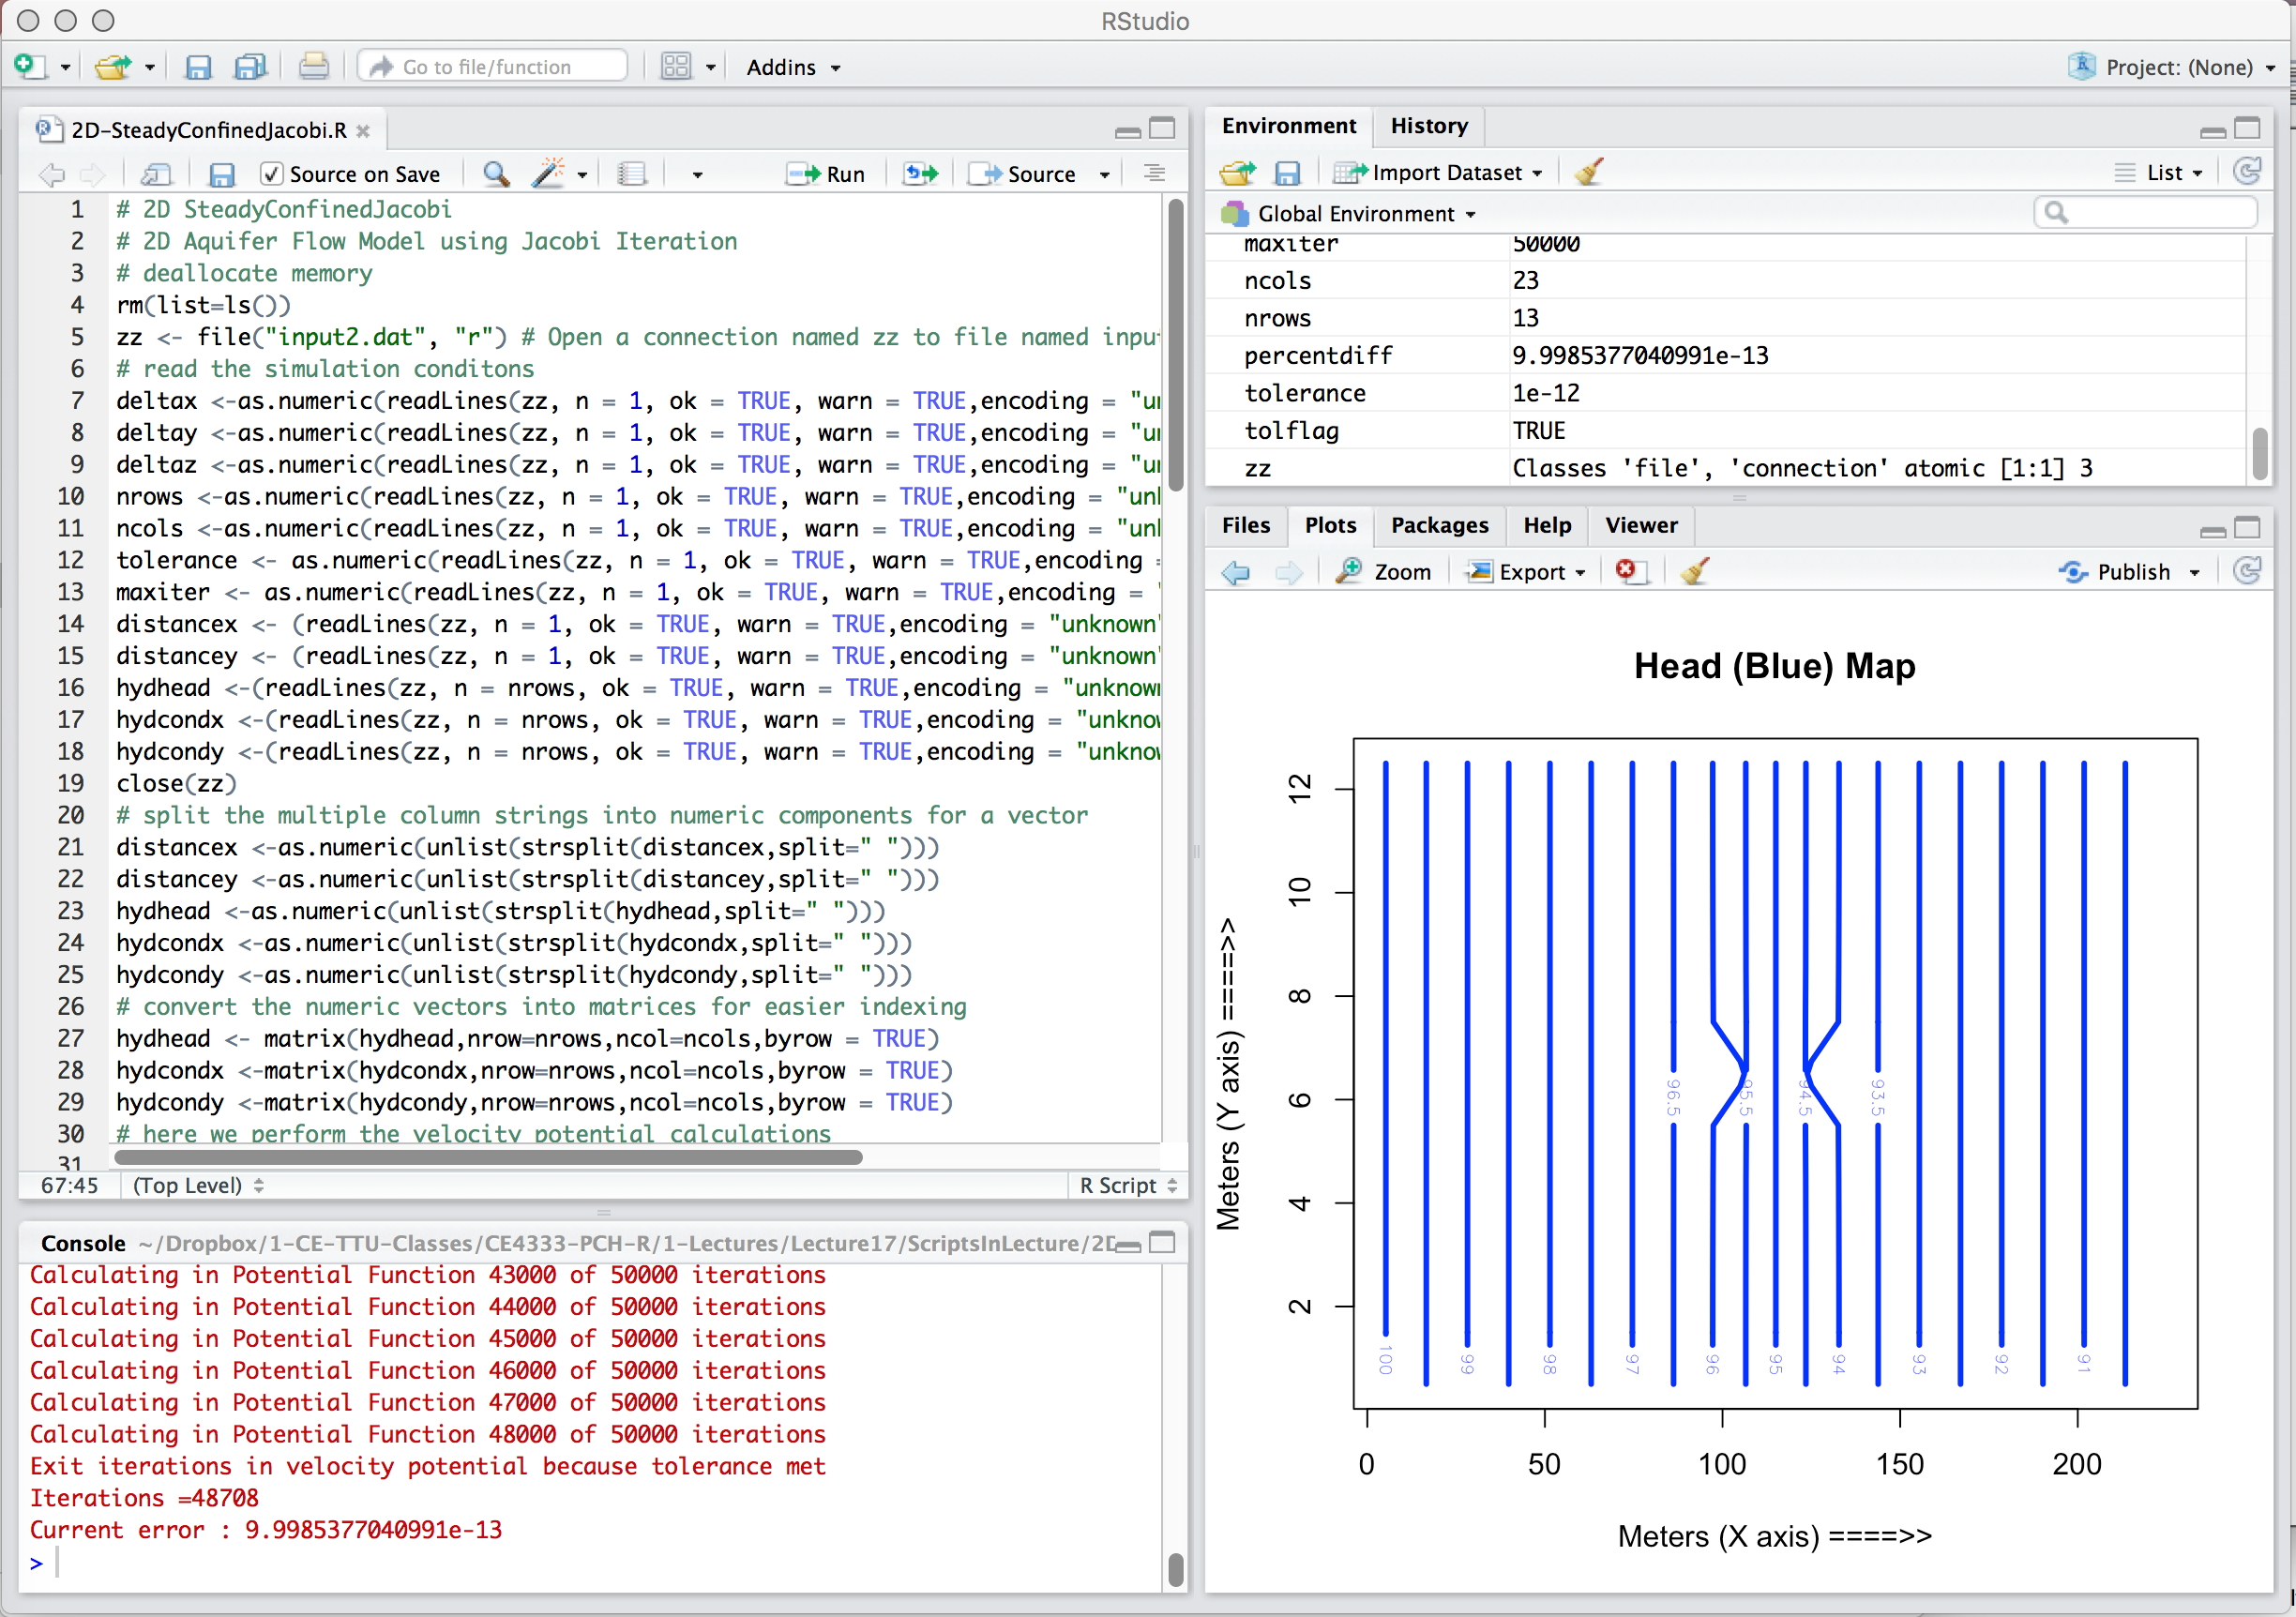
\includegraphics[width=5.2in]{./14-PorousMediumFlow/LowPInclusionOut.jpg} 
   \caption{Vertical slice in an aquifer with low permeability inclusion using Jacobi iteration scripts}
   \label{fig:LowPInclusionOut}
\end{figure}

[Modifications to handle generalized boundary conditions]



\clearpage
\subsection{Unconfined Aquifer Flow}
\subsubsection{Finite-Difference Methods}
\subsection{Exercises}
%%%%%%%%%%%%%%%%%%%%%%%%%%%%%%%%%%%%%%%%%%%%%%%%%%%%%%